%  The AAU Poster Theme.
%  2013-05-08 v. 1.1.0
%  Copyright 2013 by Jesper Kjær Nielsen <jkn@es.aau.dk>
%
%  This is free software: you can redistribute it and/or modify
%  it under the terms of the GNU General Public License as published by
%  the Free Software Foundation, either version 3 of the License, or
%  (at your option) any later version.
%
%  This is distributed in the hope that it will be useful,
%  but WITHOUT ANY WARRANTY; without even the implied warranty of
%  MERCHANTABILITY or FITNESS FOR A PARTICULAR PURPOSE.  See the
%  GNU General Public License for more details.
%
%  You can find the GNU General Public License at <http://www.gnu.org/licenses/>.
%\documentclass[a0paper, portrait]{Julam_Korea}
\documentclass[Junlampaper, portrait]{Junlam_PosterK}
\usepackage{kotex}
\usepackage[english]{babel}
\usepackage{helvet}
\renewcommand{\familydefault}{\sfdefault} % for text
\usepackage[helvet]{sfmath} % for math
\usepackage[T1]{fontenc}
\usepackage{algpseudocode} 
\usepackage{cite}

\usepackage{caption}
\captionsetup{
  font=tiny, % set font size to footnotesize
  labelfont=bf % bold label (e.g., Figure 3.2) font
    }
% Make the standard latex tables look so much better
\usepackage{array,booktabs}
% For creating beautiful plots
\usepackage{pgfplots}

\usepackage{amsmath}
% Adds new math symbols
\usepackage{amssymb}
\usepackage{algorithm}
\usepackage{tikz}
\usepackage{pgfplots}
\usepackage{filecontents}
\usepackage{pgfplotstable}
\pgfplotsset{
	compat=newest,
	% label style={font=\scriptsize},
	% ticklabel style={font=\scriptsize},
	% legend style={font=\tiny},
	% major tick length=0.1cm,
	% minor tick length=0.05cm,
	% every x tick/.style={black},
}

\definecolor{mygreen}{rgb}{0,0.6,0}
\definecolor{mygray}{rgb}{0.47,0.47,0.33}
\definecolor{myorange}{rgb}{0.8,0.4,0}
\definecolor{mywhite}{rgb}{0.98,0.98,0.98}
\definecolor{myblue}{rgb}{0.01,0.61,0.98}

\usepackage{listings}
\lstset{
	basicstyle=\small\ttfamily,
	columns=flexible,
	breaklines=true
}
%% language specific settings:
\lstdefinestyle{Arduino}{%
    style=FormattedNumber,
    keywords={void},%                 define keywords
    morecomment=[l]{//},%             treat // as comments
    morecomment=[s]{/*}{*/},%         define /* ... */ comments
    emph={HIGH, OUTPUT, LOW},%        keywords to emphasize
}
%% language specific settings:
\lstdefinestyle{Arduino}{%
    style=FormattedNumber,
    keywords={void},%                 define keywords
    morecomment=[l]{//},%             treat // as comments
    morecomment=[s]{/*}{*/},%         define /* ... */ comments
    emph={HIGH, OUTPUT, LOW},%        keywords to emphasize
}

%%%%%%%%%%%%%%%%%%%%%%%%%%%%%%%%%%%%%%%%%%%%%%%%
% Colours
% http://en.wikibooks.org/wiki/LaTeX/Colors
%%%%%%%%%%%%%%%%%%%%%%%%%%%%%%%%%%%%%%%%%%%%%%%%
\selectcolormodel{RGB}
% define the three aau colors : blue version
\definecolor{aaublue1}{RGB}{33,26,82}% dark blue
\definecolor{aaublue2}{RGB}{113,109,143} % light blue
\definecolor{aaublue3}{RGB}{194,193,204} % lighter blue


%green 
%\definecolor{aaublue1}{RGB}{0,163,136}% dark green
%\definecolor{aaublue2}{RGB}{121,189,143} % light green
%\definecolor{aaublue3}{RGB}{190,235,159} % lighter green
%\definecolor{aaublue4}{RGB}{255,255,157} % yellow
%\definecolor{aaublue5}{RGB}{255,97,56}


%%%%%%%%%%%%%%%%%%%%%%%%%%%%%%%%%%%%%%%%%%%%%%%%
% Lists
% http://en.wikibooks.org/wiki/LaTeX/List_Structures
%%%%%%%%%%%%%%%%%%%%%%%%%%%%%%%%%%%%%%%%%%%%%%%%
% Easier configuration of lists
\usepackage{enumitem}
%configure itemize
\setlist{%
  topsep=0pt,% set space before and after list
  noitemsep,% remove space between items
  labelindent=\parindent,% set the label indentation to the paragraph indentation
  leftmargin=*,% remove the left margin
  font=\color{aaublue1}\normalfont, %set the colour of all bullets, numbers and descriptions to aaublue1
}
% use set<itemize,enumerate,description> if you have an older latex distribution
\setitemize[1]{label={\raise1.25pt\hbox{$\blacktriangleright$}}}
\setitemize[2]{label={\scriptsize\raise1.25pt\hbox{$\blacktriangleright$}}}
\setitemize[3]{label={\raise1.25pt\hbox{$\star$}}}
\setitemize[4]{label={-}}
%\setenumerate[1]{label={\theenumi.}}
%\setenumerate[2]{label={(\theenumii)}}
%\setenumerate[3]{label={\theenumiii.}}
%\setenumerate[4]{label={\theenumiv.}}
%\setdescription{font=\color{aaublue1}\normalfont\bfseries}

% use setlist[<itemize,enumerate,description>,<level>] if you have a newer latex distribution
%\setlist[itemize,1]{label={\raise1.25pt\hbox{$\blacktriangleright$}}}
%\setlist[itemize,2]{label={\scriptsize\raise1.25pt\hbox{$\blacktriangleright$}}}
%\setlist[itemize,3]{label={\raise1.25pt\hbox{$\star$}}}
%\setlist[itemize,4]{label={-}}
%\setlist[enumerate,1]{label={\theenumi.}}
%\setlist[enumerate,2]{label={(\theenumii)}}
%\setlist[enumerate,3]{label={\theenumiii.}}
%\setlist[enumerate,4]{label={\theenumiv.}}
%\setlist[description]{font=\color{aaublue1}\normalfont\bfseries}

%%%%%%%%%%%%%%%%%%%%%%%%%%%%%%%%%%%%%%%%%%%%%%%%
% Misc
%%%%%%%%%%%%%%%%%%%%%%%%%%%%%%%%%%%%%%%%%%%%%%%%
% change/remove some names
\addto{\captionsenglish}{
  %remove the title of the bibliograhpy
  \renewcommand{\refname}{\vspace{-0.7em}}
  %change Figure to Fig. in figure captions
  \renewcommand{\figurename}{\tiny{Fig.}}
}
% create links
\usepackage{url}
%note that the hyperref package is currently incompatible with the baposter class

%%%%%%%%%%%%%%%%%%%%%%%%%%%%%%%%%%%%%%%%%%%%%%%%
% Macros
%%%%%%%%%%%%%%%%%%%%%%%%%%%%%%%%%%%%%%%%%%%%%%%%
\newcommand{\alert}[1]{{\color{aaublue1}#1}}
%%%%%%%%%%%%%%%%%%%%%%%%%%%%%%%%%%%%%%%%%%%%%%%%
% Document Start 
%%%%%%%%%%%%%%%%%%%%%%%%%%%%%%%%%%%%%%%%%%%%%%%%
\begin{document}
%%%%%%%%%%%%%%%%%%%%%%%%%%%%%%%%%%%%%%%%%%%%%%%%
% Some changes that cannot be made in the preamble
%%%%%%%%%%%%%%%%%%%%%%%%%%%%%%%%%%%%%%%%%%%%%%%%
% set the background of the poster
% \background{
%   \begin{tikzpicture}[remember picture,overlay]%
%     %the poster background color
%     \fill[fill=aaublue3] (current page.north west) rectangle (current page.south east);
%     %the header
%     \fill [fill=aaublue1] (current page.north west) rectangle ([yshift=-\headerheight] current page.north east);
%   \end{tikzpicture}
% }
\background{
    \begin{tikzpicture}[remember picture, overlay, anchor=south west, inner sep=0pt]%
        \node at (-1.2, -0.65)  %(16.30, 18.40) 
                 {\includegraphics[width=\paperwidth, height=\paperheight]
                {wallpaper/wallpaper4.pdf}};
    % \end{tikzpicture}
    % \begin{tikzpicture}[remember picture, overlay]%
        %\node [draw, width=13cm, height=3cm, text=black] (abs) at (1.6, 28.2) 
            %{\tiny{해안, 연안 등을 소규모로 재현하여 연안 공학, 선박 공학 등의 분야와 관련된 모형 실험이 가능한 2차원 조파 수조를 제작하였다. 조파 수조는 수조 모듈, 조파기, 소파기, 파고계, 경사로(연안 모형)으로 구성된다. 수조 모듈은 길이 $2,000~\mathrm{mm}$, 폭 $300~\mathrm{mm}$, 높이 $400~\mathrm{mm}$이며 3개로 연결하여 길이 $6,000~\mathrm{mm}$로 구성하였다. 조파기는 구동부와 제어부로 나뉘며, 구동부는 리니어 엑츄에이터와 스텝 모터를 주 부품으로 하고, 이를 제어부의 틴시 보드 기반 컨트롤러로 제어한다. 개발한 아두이노 코드로 조파기를 구동시켜 여러 파를 발생시킬 수 있고, 이에 의한 맞춤형 파 생성이 가능하여 원하는 조건에 대한 모형 실험을 구현할 수 있다.}};
        \node at (4.1, 30.9) 
            {
\includegraphics[width=4cm, height=4cm]
                {images/number.png}};
        \node [inner sep=0pt] at (26.0, 26.8) 
            {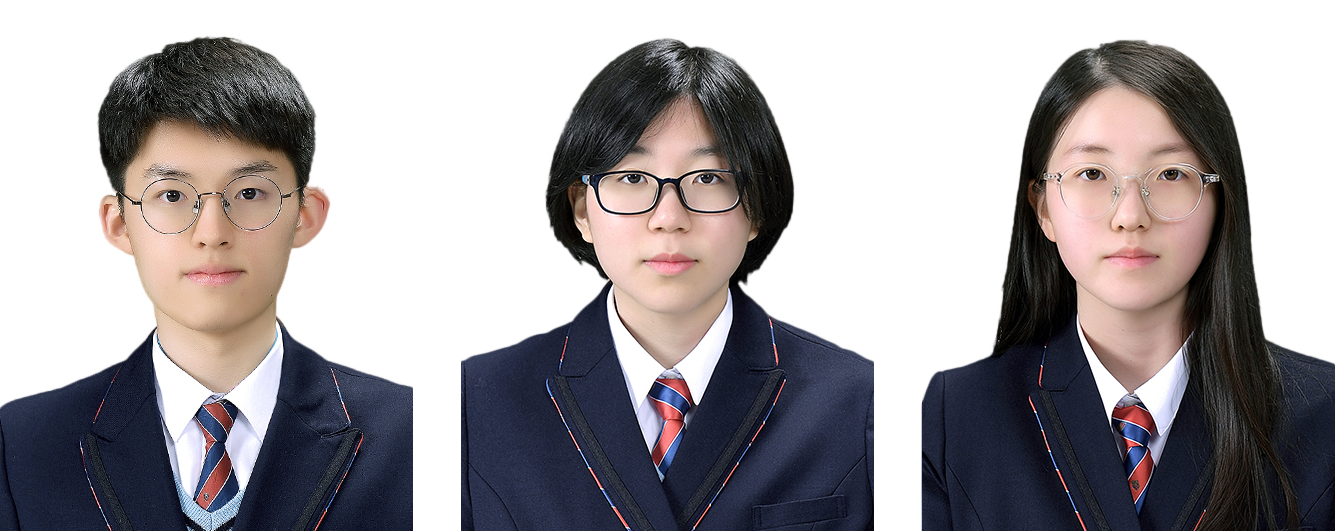
\includegraphics[width=6.8cm]
                {./photo/3_photo.png}};
        
        \node [text=green] (students) at (20.5, 28.9) {\bf \LARGE{출 품 자 : }}; %at (가로, 세로)
        \node [text=black] (studentsname1) at (23.5, 28.9) {\bf \LARGE{남도현}}; 
        \node [text=black] (studentsname2) at (23.5, 28.2) {\bf \LARGE{백효송}}; 
        \node [text=black] (studentsname3) at (23.5, 27.5) {\bf \LARGE{이시현}}; 
        \node [text=green] (advisor) at (20.5, 26.8) {\bf \LARGE{지도교사: }};
        \node [text=black] (advisorname) at (23.5, 26.8) {\bf \LARGE{박기현}};
    \end{tikzpicture}
}
% if you want to reduce the space before and after equations, use and adjust
% the following lines
%\addtolength{\abovedisplayskip}{-2mm}
%\addtolength{\belowdisplayskip}{-2mm}

%%%%%%%%%%%%%%%%%%%%%%%%%%%%%%%%%%%%%%%%%%%%%%%%
% General poster setup
%%%%%%%%%%%%%%%%%%%%%%%%%%%%%%%%%%%%%%%%%%%%%%%%
\begin{poster}{
  %general options for the poster
  grid=false,
  columns=4, #
  colspacing=3mm,
  headerheight=0.33\textheight,
  background=user,
%  bgColorOne=red!42, %is used when background != user and none
%  bgColortwo=green!42, %is used when background is shaded
  eyecatcher=true,
  %posterbox options
  headerborder=closed,
  borderColor=aaublue1,
  headershape=rectangle,
  headershade=plain,
  headerColorOne=aaublue1,
%  headerColortwo=yellow!42, %is used when the header background is shaded
  textborder=rectangle,
  boxshade=plain,
  boxColorOne=white,
%  boxColorTwo=cyan!42,%is used when the text background is shaded
  headerFontColor=white,
  headerfont=\Large\sf\bf,
  linewidth=1pt
}

%the Eye Catcher (the logo on the left)
{
  % This can be commented out or replaced by a company/department logo
  %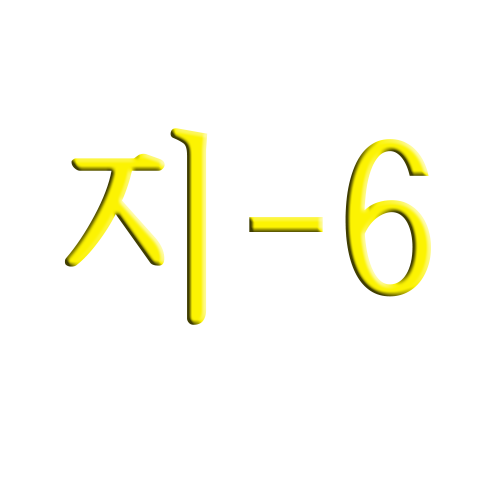
\includegraphics[height=0.3\headerheight]{images/gshslogo1.png}
}
%the poster title
{
%\vspace{-10em} \quad \quad \color{blue}\HUGE{연안 환경 모형 실험을 위한 2차원 조파 수조 제작}
}
%the author(s)
%{
 %{}
%}
%the logo (the logo on the right)
%{
  % This can be commented out or replaced by a company/department logo
  %\includegraphics[height=0.3\headerheight]{./logo/gshslogo.png}
%}

%%%%%%%%%%%%%%%%%%%%%%%%%%%%%%%%%%%%%%%%%%%%%%%%
% The actual content of the poster begins here
%%%%%%%%%%%%%%%%%%%%%%%%%%%%%%%%%%%%%%%%%%%%%%%%

% \begin{posterbox}[name=abstra,span=2,column=0,row=0]{Abstract}
%   \scriptsize{
%   해안, 연안 등을 소규모로 재현하여 연안 공학, 선박 공학 등의 분야와 관련된 모형 실험이 가능한 2차원 조파 수조를 제작하였다. 조파 수조는 수조 모듈, 조파기, 소파기, 파고계, 경사로(연안 모형)으로 구성된다. 수조 모듈은 길이 $2,000~\mathrm{mm}$, 폭 $300~\mathrm{mm}$, 높이 $400~\mathrm{mm}$이며 3개로 연결하여 길이 $6,000~\mathrm{mm}$로 구성하였다. 조파기는 구동부와 제어부로 나뉘며, 구동부는 리니어 엑츄에이터와 스텝 모터를 주 부품으로 하고, 이를 제어부의 틴시 보드 기반 컨트롤러로 제어한다. 개발한 아두이노 코드로 조파기를 구동시켜 여러 파를 발생시킬 수 있고, 이에 의한 맞춤형 파 생성이 가능하여 원하는 조건에 대한 모형 실험을 구현할 수 있다.
%   }
% \end{posterbox}

\begin{posterbox}[name=intro,column=0]{서론}
    \small {1. 제작 동기 \\}
        \scriptsize {
        연구를 계획하던 중 모형 실험을 위하여 연안 모형과 이곳에 해파를 발생시키는 장치가 필요하게 되었다. 선행 연구를 조사해 보니 연안 등 다양한 조건에서 해양 현상의 모의 실험은 조파 수조를 이용하여 할 수 있다는 것을 알게 되었다\cite{chung2013}.\\}

    \small {2. 제작 목적\\} 
        \scriptsize {
        본 조파 수조는 파도를 발생시키거나 이를 이용한 모형 실험을 하기 위하여 개발되었다. 
          \begin{itemize}
            \item 쓰나미에 의한 피해를 알아보는 연안의 구조물 모형 실험
            \item 다양한 파력발전 모형 실험
            \item 방파제의 조적구조 효율 비교 실험
            \item 선박, 부표 등의 안정성 비교 실험
          \end{itemize}
          }
        \end{posterbox}

\begin{posterbox}[name=theo,column=0,below=intro]{이론적 배경}
   \small {1. 2차원 조파 수조\\} %조파기 \\
     \scriptsize {조파 수조는 모형 실험용 수조로 해안 혹은 연안에서의 여러 현상을 축소하여 재현 및 실험하기 위한 장치이다. 소규모로 운영이 용이하며 정확한 파를 생성하고 변화를 관찰하기 위해서는 파의 진행방향이 한 방향인 2차원 조파 수조가 적합하다. \\}
     
   \small {2. Wave Maker Theory\\}
     \scriptsize {
     2차원 조파 수조에서는 유체와 관련된 여러 방정식과 경계조건을 도입하여 근사적인 파의 개형을 얻을 수 있다. 심해파 조건에서는 파가 다음과 같이 표현된다. \cite{ART002413750, ART002785404, dean1991water}.
      \begin{equation*}
         \mu(x,t)=\frac{H}{2}\cos(kx-\sigma t),~\frac{H}{S_0}=\frac{4\sinh^2 kh}{\sinh kh + 2kh}
      \end{equation*}
         $S_0$는 스트로크이며 Froude 상사 법칙에 의하면 $\omega \sim 4\pi$ 정도는 되어야 심해파 조건을 만족하여 제대로 된 $\sin$파가 생성될 수 있다.}
 \vspace{0.8em}
\end{posterbox}


\begin{posterbox}[name=wtank,span=2,column=1,row=0] {작품 설명: A. 2차원 조파 수조 (길이 확장 가능)}
%\begin{figure}[H]
        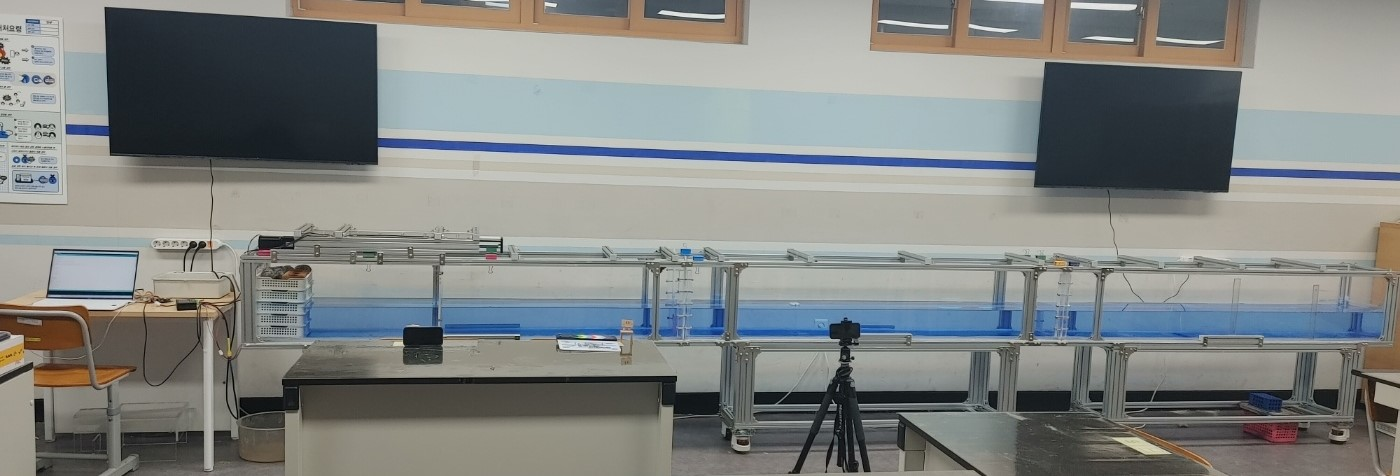
\includegraphics[width=\textwidth]{images/Experiment_System_Crop}
        \captionof{figure}{완성된 조파수조의 모습}
 %       \label{Experimnet_System} 
        \begin{tikzpicture} [remember picture, overlay, anchor=north west]
            \node [draw=yellow, text=yellow] (TV1) at (2.4, 5.8) {\scriptsize{TV1}};
            \node [draw=yellow, text=yellow] (TV2) at (12.4, 5.5) {\scriptsize{TV2}};
            \node [draw=yellow, text=yellow] (computer) at (1.0, 4) {\scriptsize{computer}};
            \node [draw=yellow, text=yellow] at (4.6, 2.6) {\scriptsize{camera1}};
            \node [draw=yellow, text=yellow] at (9.5, 2.5) {\scriptsize{camera2}}; 
        \end{tikzpicture}
        %\captionof{figure}{\scriptsize 완성된 조파 수조의 모습} %\\[0.5em]\
%\end{figure}
\newline
\scriptsize 제작한 작품은 '2차원 조파 수조'로 명명하였다. 이 조파 수조를 이용하여 실험을 할때 제대로 진행이 되려면 조파기, 소파기, 파고계, 해안 경사로 등이 제 역할을 해 주어야 가능하다. 따라서 각 부분은 실험 목적에 따라 조립과 분해가 가능하도록 따로 제작하였다. 제작한 조파 수조의 특징을 나열하면 다음과 같다.
\begin{itemize}
    \item 폭 $300~\mathrm{mm}$, 높이 $400~\mathrm{mm}$, 총 길이 $6,000~\mathrm{mm}$의 2차원 조파 수조를 제작하였다. 폭과 높이를 맞추어 수조 모듈을 추가로 제작하여 연결하면 얼마든지 길이를 확장할 수 있다.
    \item 수조는 3030, 3060 알루미늄 프로파일을 이용하여 틀을 제작한 후, 그 안에 아크릴 판을 넣고 접착제로 붙인 후 실리콘으로 물이 새지 않도록 조치하였다.  
    \item 조파기의 구동부는 리니어 엑츄레이터에 아크릴 판을 부착하여 물을 밀어낼 수 있도록 설계하였고 스텝 모터가 회전하면 조파판이 앞, 뒤로 움직이는 구조이다.
    \item 조파기의 제어보는 틴지 보드를 기반으로 하여 회로를 설계하였으며 스텝 모터 드라이버를 이용하여 모터를 움직이도록 하였다. 
    \item 조파판과 조파 수조 사이에서 틈이 최소가 되도록 조파판의 크기를 설계하여 부착하였다. 
    \item 양 끝이 막혀 있는 수조에서 정상파가 생기거나 반사파에 의한 간섭을 줄이기 위하여 철 수세미를 이용하여 소파 장치를 만들었다. 
    \item 현재 조파기를 이용하여 규칙파를 생성할 수 있는 코드가 완성되었으며 이후 쓰나미 등의 불규칙파를 생성하거나 정교한 제어를 할 수 있도록 코드를 업그레이드 할 예정이다. 
    \item 해안 경사로는 교각 위에 아크릴 판을 올리는 구조로 설계하여 길이와 기울기를 변화시켜 탈부착이 가능하도록 제작하였다. 
    \item 파고계는 물에 잘 뜨는 재질로 제작하여 동영상 분석을 통해 파고를 파악하고 있으며, 이후 센서를 부착하여 정밀한 파고를 측정하도록 개선할 예정이다.
\end{itemize}

        % 수조는 모듈 3개로 구성되어 있다. 단일 모듈은 길이 $2,000~\mathrm{mm}$, 폭 $300~\mathrm{mm}$, 높이 $400~\mathrm{mm}$며 기본 프레임은 알루미늄 프로파일이다. 내부 벽은 아크릴이고 실리콘 패드를 'ㄷ'자 모양으로 잘라 모듈 사이에 끼운다. 아크릴 판의 옆, 아래에는 아크릴 막대를 붙여 밀착시키고 볼트를 이용하여 고정한다. 마지막으로 실리콘 칠을 하여 틈새를 마감한다. \\
        % 수조의 양 끝에는 소파기를 설치하였다. 조파판 뒷쪽에는 구멍이 뚫린 플라스틱 바구니에 철수세미를 넣어 쌓음으로써 만든 소파 장치를 설치하였으며 그 반대쪽에는 3D프린터로 제작한 다공성 소파장치와 플라스틱 바구니를 이용해 만든 소파 장치를 모두 설치하였다. \\
        % 수조에서 조파기가 위치한 쪽의 반대쪽에는 경사로를 설치할 수 있다. 경사로는 아크릴 판을 이용해 만들었으며 알루미늄 프로파일로 지지대를 만들었다. 경사로는 높이 $200\mathrm{~mm}$, 길이 $2,000\mathrm{~mm}$로 기울기가 $1/10$ 이다. 
        
\end{posterbox}

\begin{posterbox}[name=circuit, column=0, below=theo]{작품 설명: B. 조파기-1} %, above=bottom-2000
\small {1. 구동부\\}
    \scriptsize {
    
    구동부는 알루미늄 프로파일 프레임에 $80\mathrm{~cm}$ 길이의 리니어 액츄에이터를 이용하여 제작하였다. 조파판은 액츄에이터의 이동부에 붙어 수조 내부를 수평적으로 이동하며 물이 옆부분으로 새지 않도록 공간에 딱 맞는 아크릴 판으로 제작하였다. ($295\mathrm{~mm}\times 300\mathrm{~mm} \times 15\mathrm{~mm}$).\\}
    
    %\begin{figure}[H]
            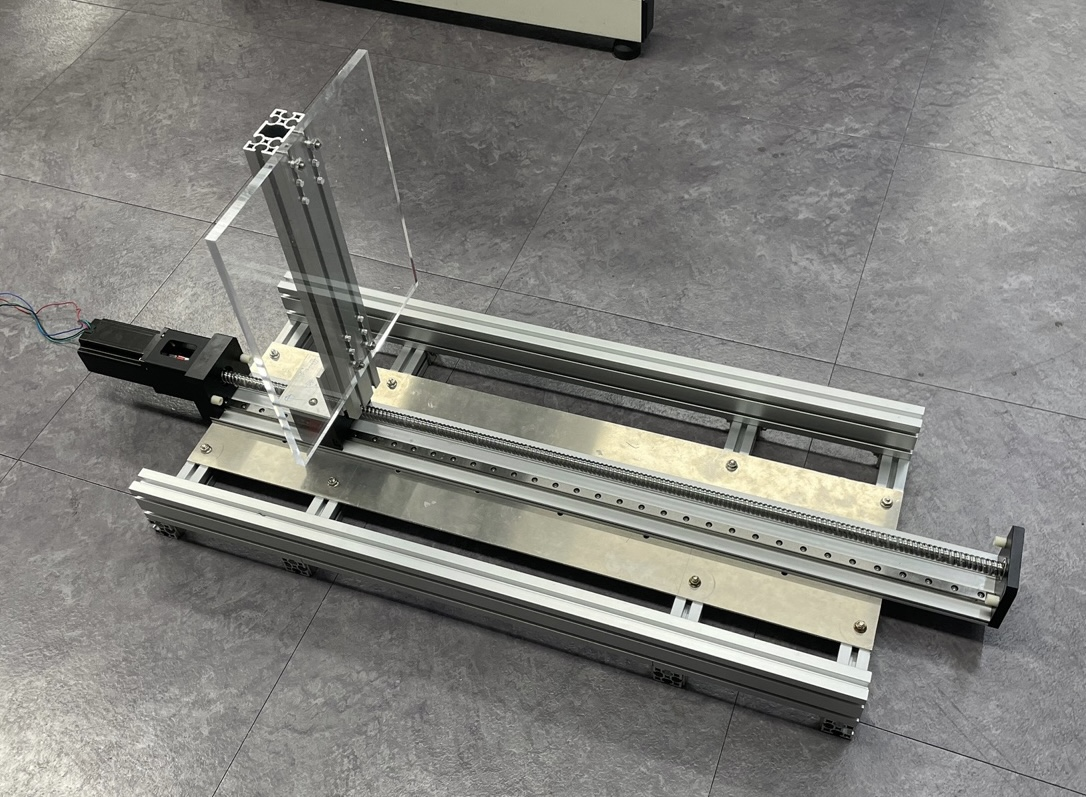
\includegraphics[width=0.42\textwidth]{images/jopagi.jpg} 
            %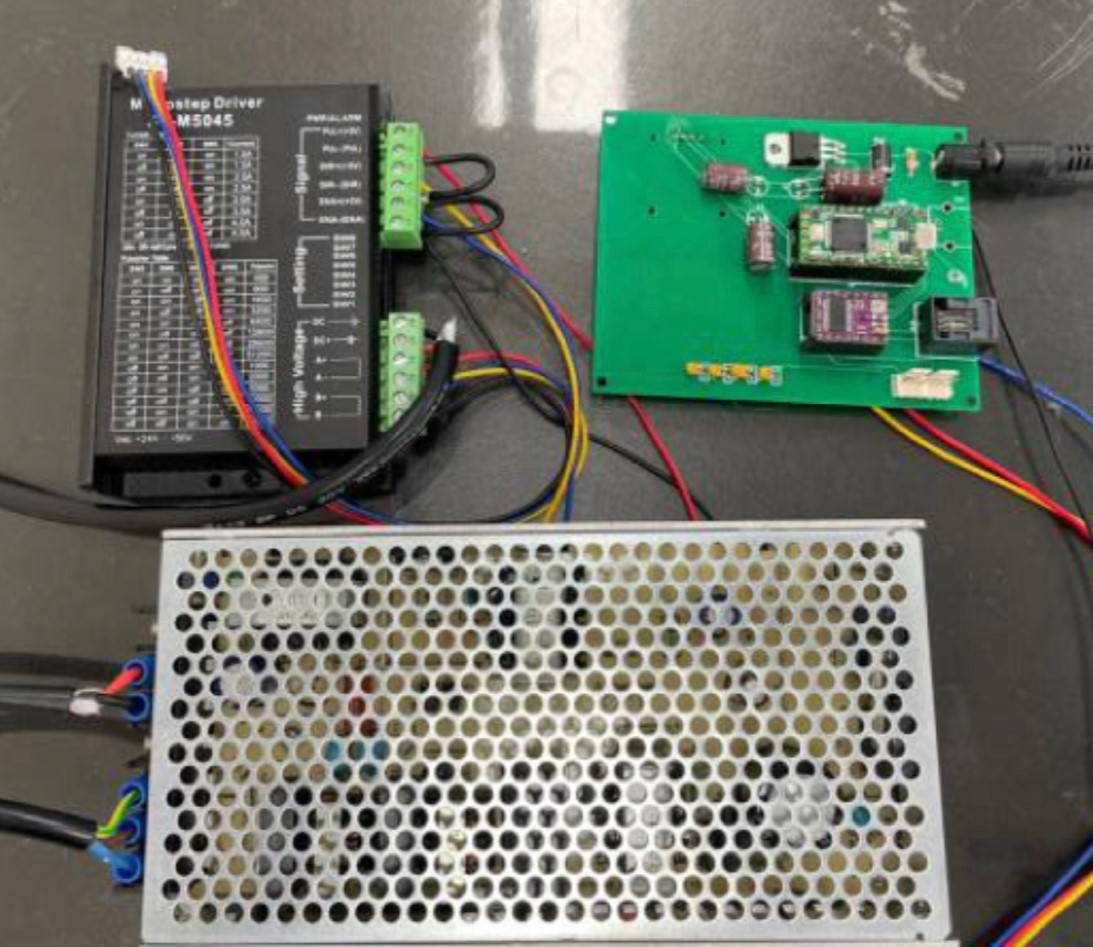
\includegraphics[width=0.465\textwidth]{images/gdb.jpg}
            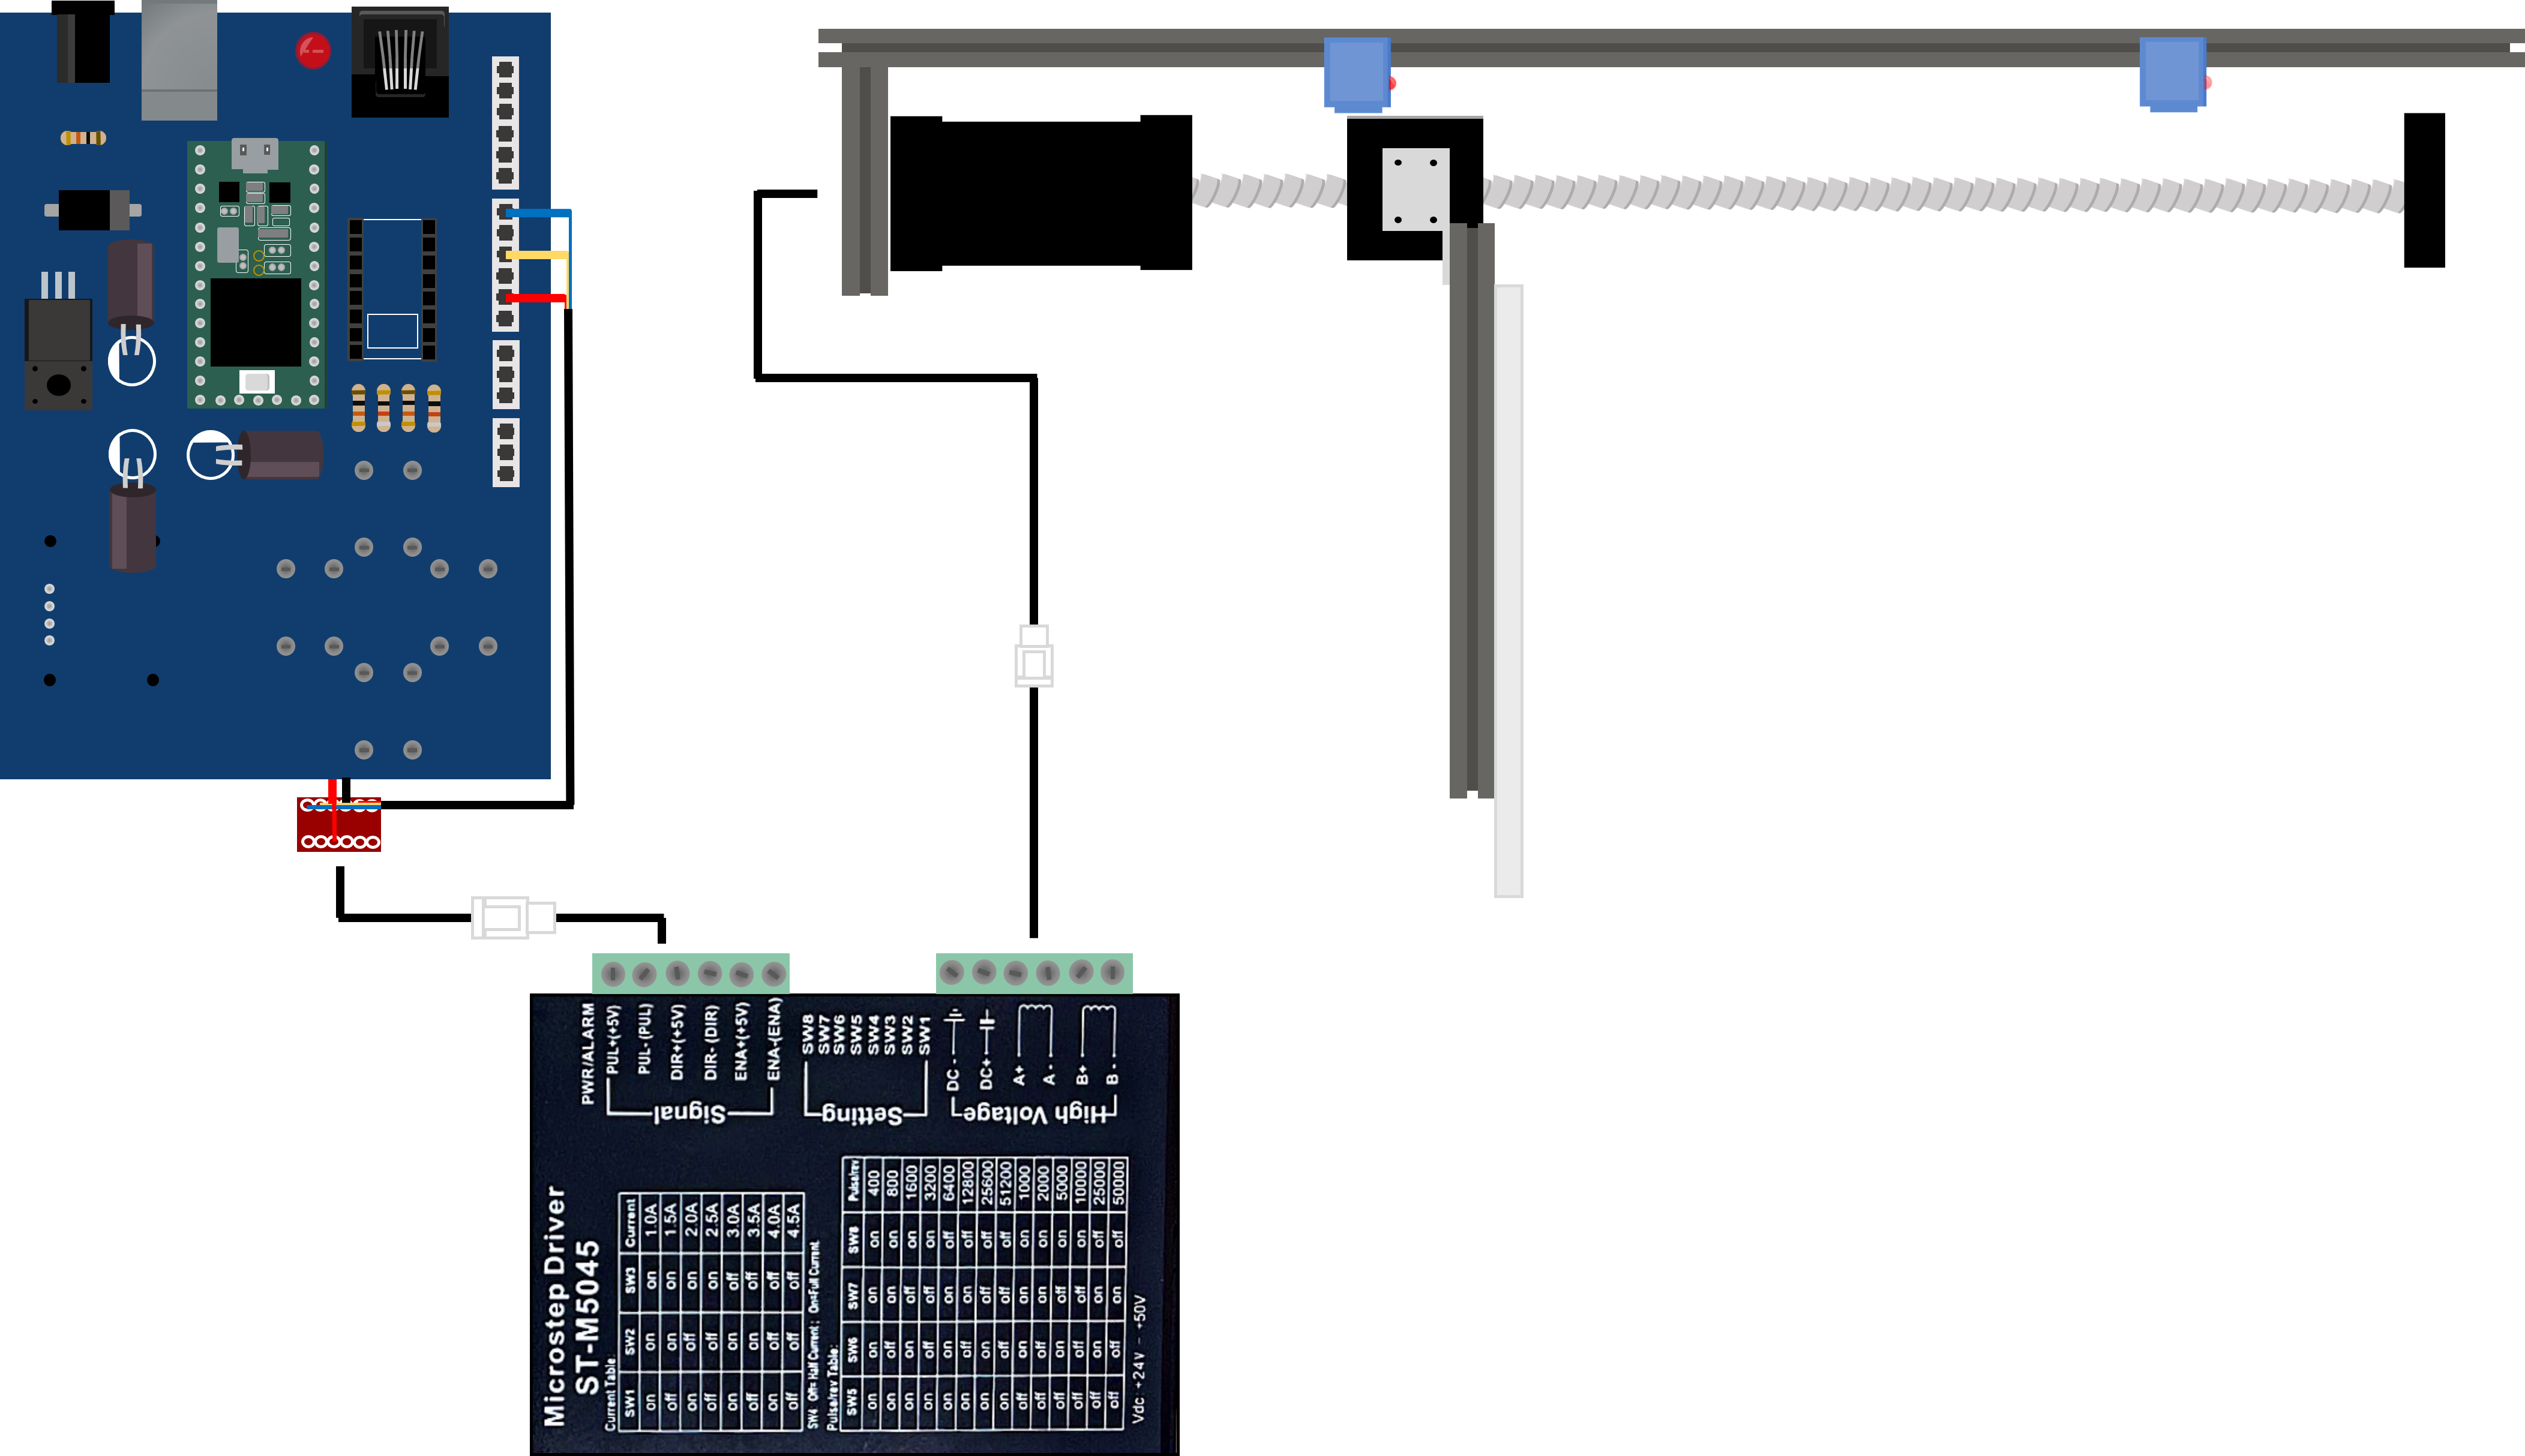
\includegraphics[width=0.52\textwidth]{images/wavemaker_control.png}
        \captionof{figure}{(a) 피스톤형 조파기의 구동부 모습과 (b) 조파기 전자 회로와 모터 드라이버, 전원장치를 연결한 모습}
        \label{circuit}   
        \begin{tikzpicture} [remember picture, overlay, anchor=north west, inner sep=0pt]
            \node [%draw=yellow, 
                    text=yellow,
                    ] at (0.1, 3.5) {\scriptsize{(a)}};
            \node [%draw=yellow, 
                    text=yellow,
                    ] at (3.5, 3.5) {\scriptsize{(b)}};
        \end{tikzpicture}	 
    %\end{figure} 

\small {2. 전자 회로부\\}
    \scriptsize {
    
    조파기의 회로는 Teensy 3.2와 DRV8825, Microstep Driver(ST-M5045), 24V SMPS로 구성되어 있다. 모터 드라이버의 최대 펄스는 400 Pulse/Rev이다. Teensy 보드와 Microstep Driver는 DIR, PULSE, ENABLE이 연결되어 있고 각각의 (-)는 보드의 Ground에 연결하였다.}
    
    %\begin{figure}[H]
            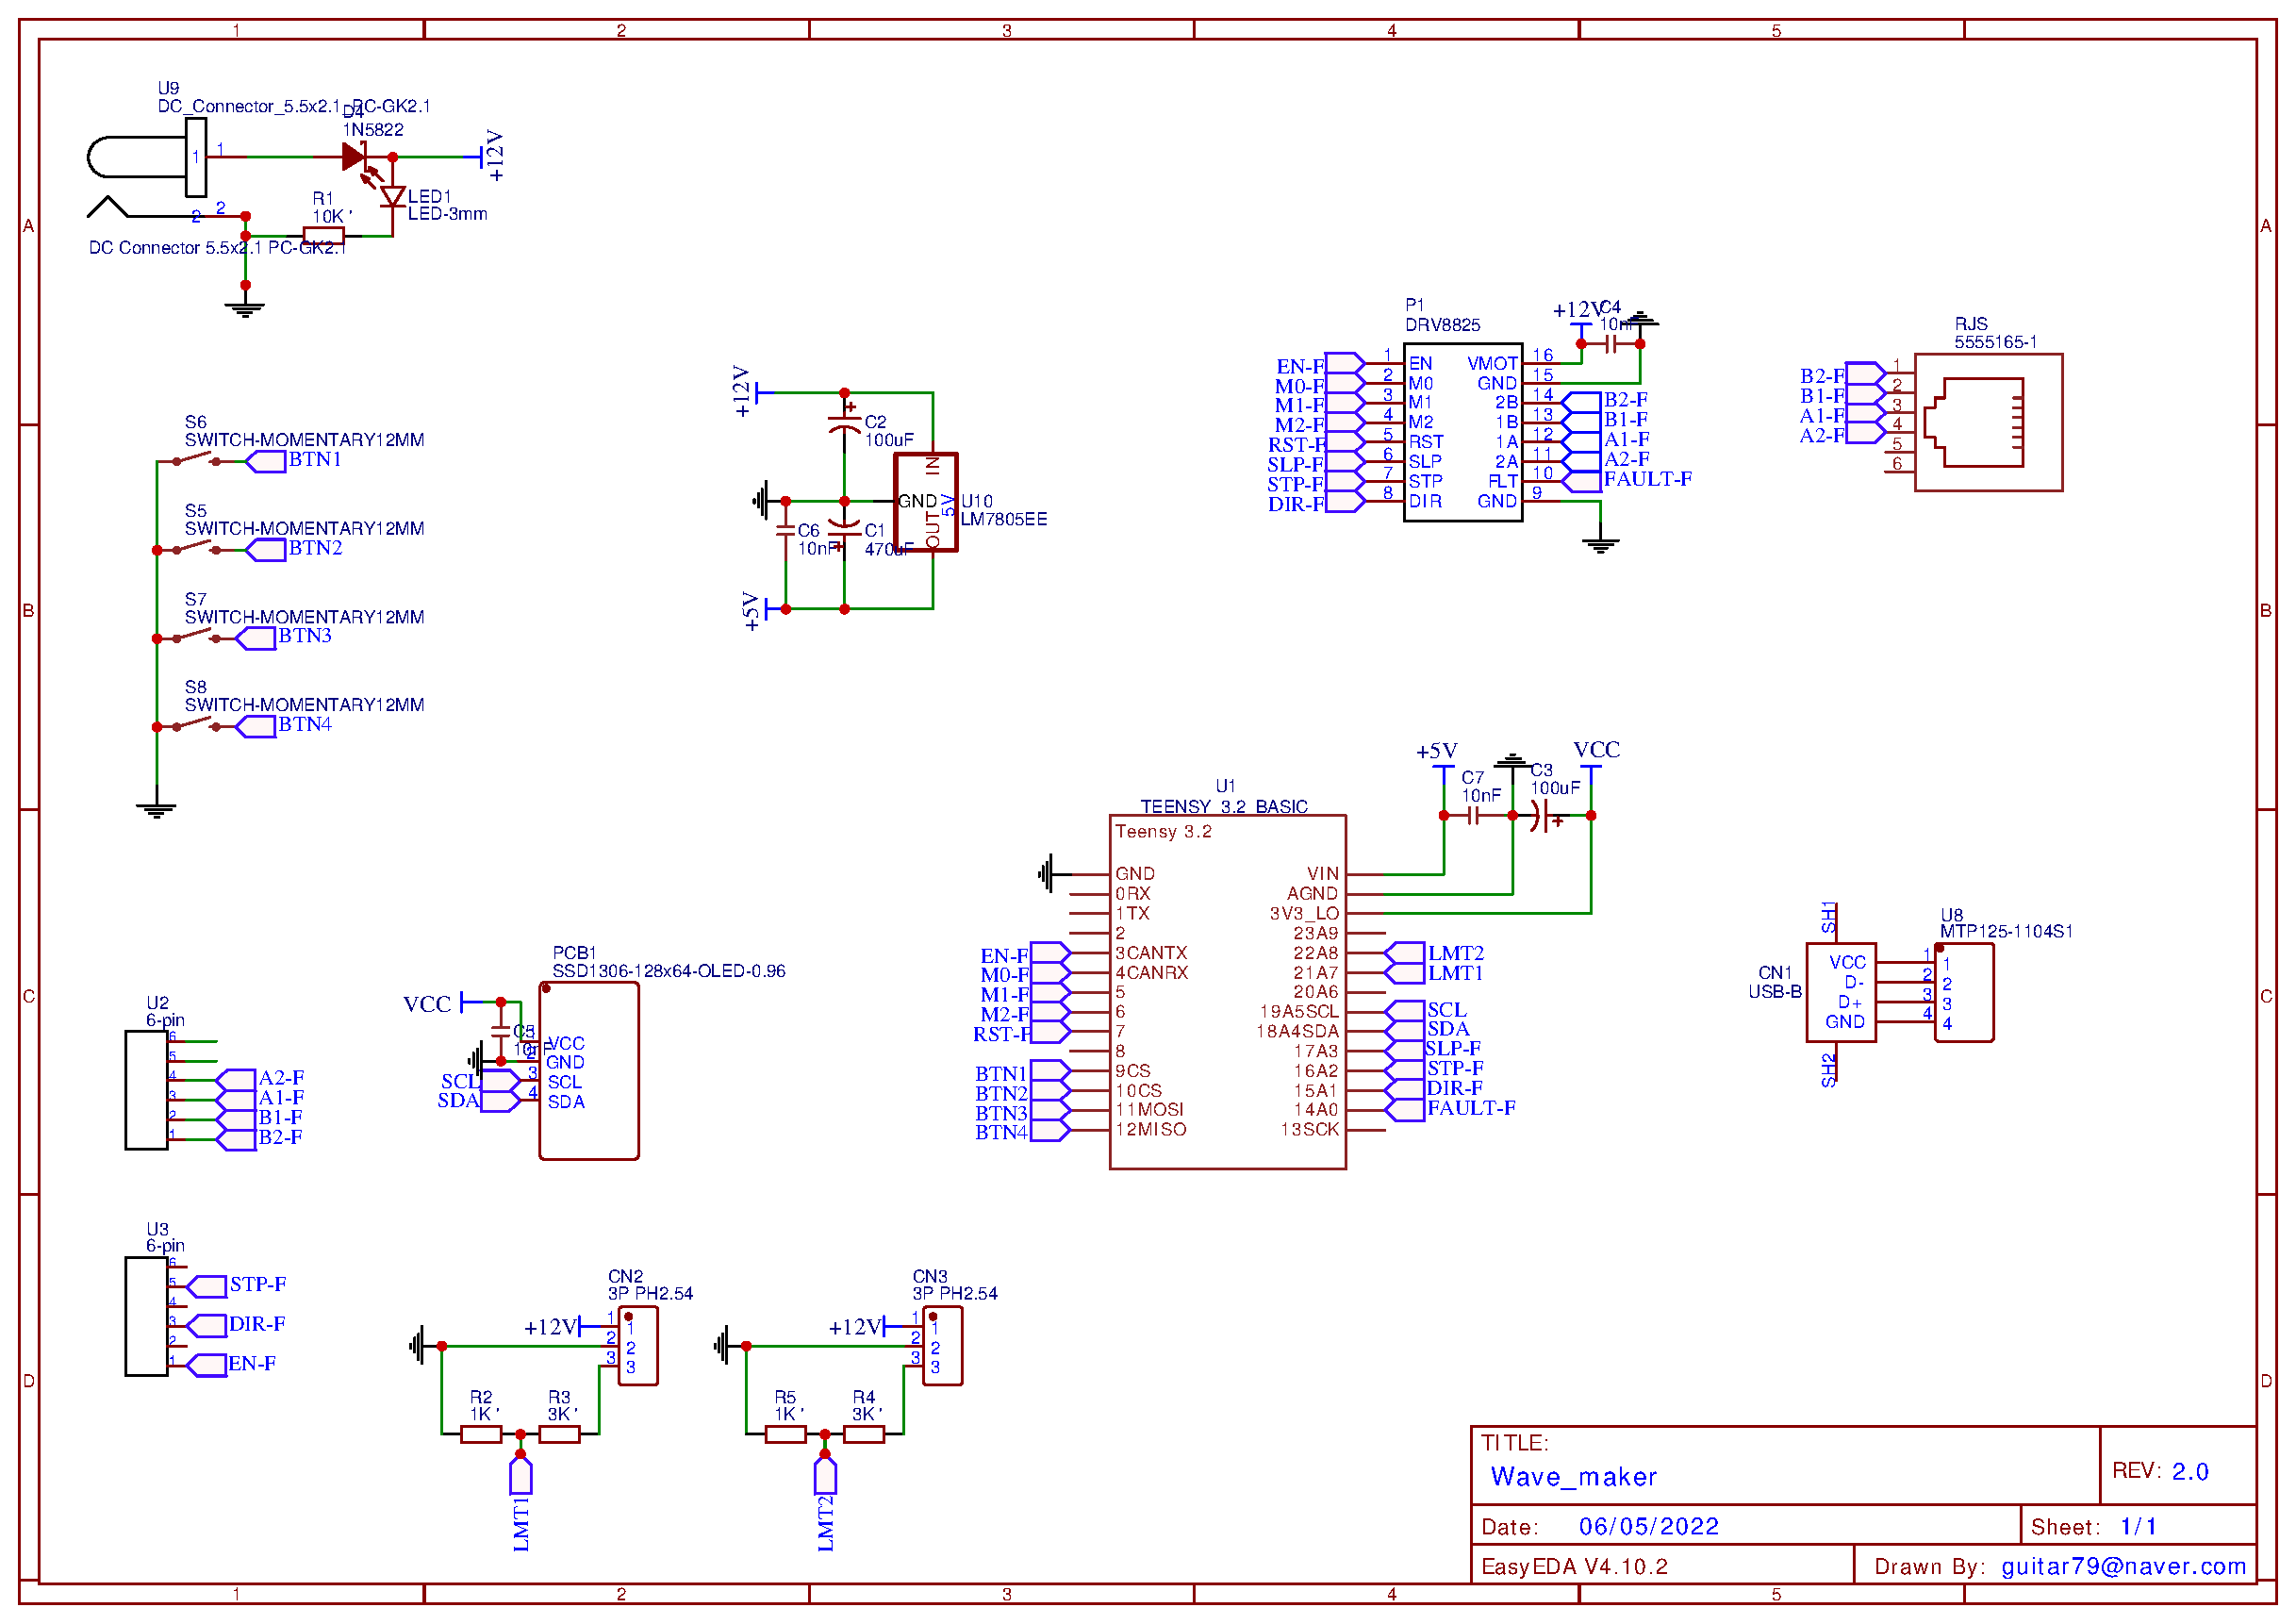
\includegraphics[width=0.52\textwidth]{images/Schematic_Wave_maker_2-1_2022-11-24.pdf}
            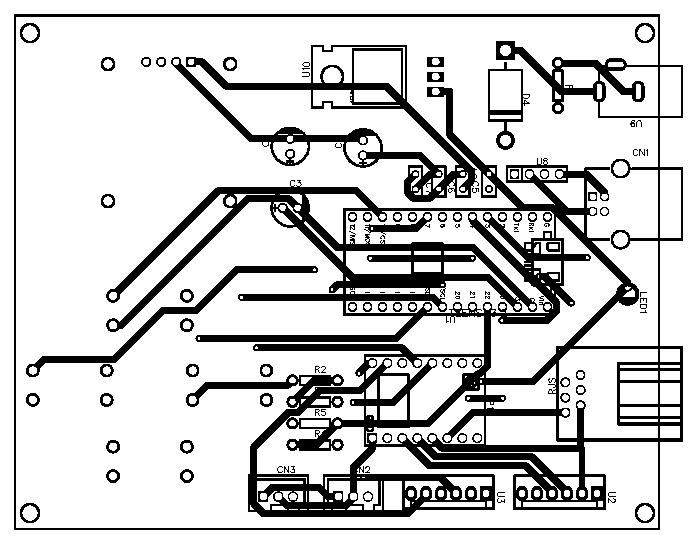
\includegraphics[width=0.47\textwidth]{images/PCB_PCB_Wave_maker copy_2022-11-24.pdf} 
            \captionof{figure}{조파기 전자 회로와 pcb 디자인}
            \label{circuit}
    %\end{figure} 
\vspace{1.0em}
\end{posterbox}

\begin{posterbox}[name=circuit,column=1,below=wtank]{작품 설명: B. 조파기-2} %, above=bottom-2000
\small {3. 코드 개발 및 컨트롤 박스 제작\\}
    \scriptsize {    
     
     모터의 빠른 구동을 위해서 TeensyStep 라이브러리를 이용하며 변위를 대입하는 방식으로 코드를 작성하였다.  변위를 대입하면 그에 맞는 속도를 계산하여 각속도를 부여하는 방식으로 모터가 작동하며 $400\mathrm{~step}$ 회전 시 1 $\rm{~cm}$ 전진한다. 이로부터 조파기가 사인형으로 움직이기 위한 코드는 다음과 같으며 변위 함수는 진폭 $A$, 각진동수 $\omega$ 등을 설정하여 조절할 수 있다.\\
     그리고 모터 구동은 모터드라이버와 함께 연결된 컨트롤 박스 하나로 가능하도록 제작하였다. ${220\rm{~V}}$ 전원을 연결하면 내부 SMPS와 12V 어뎁터에 전원이 공급된다.}
      
      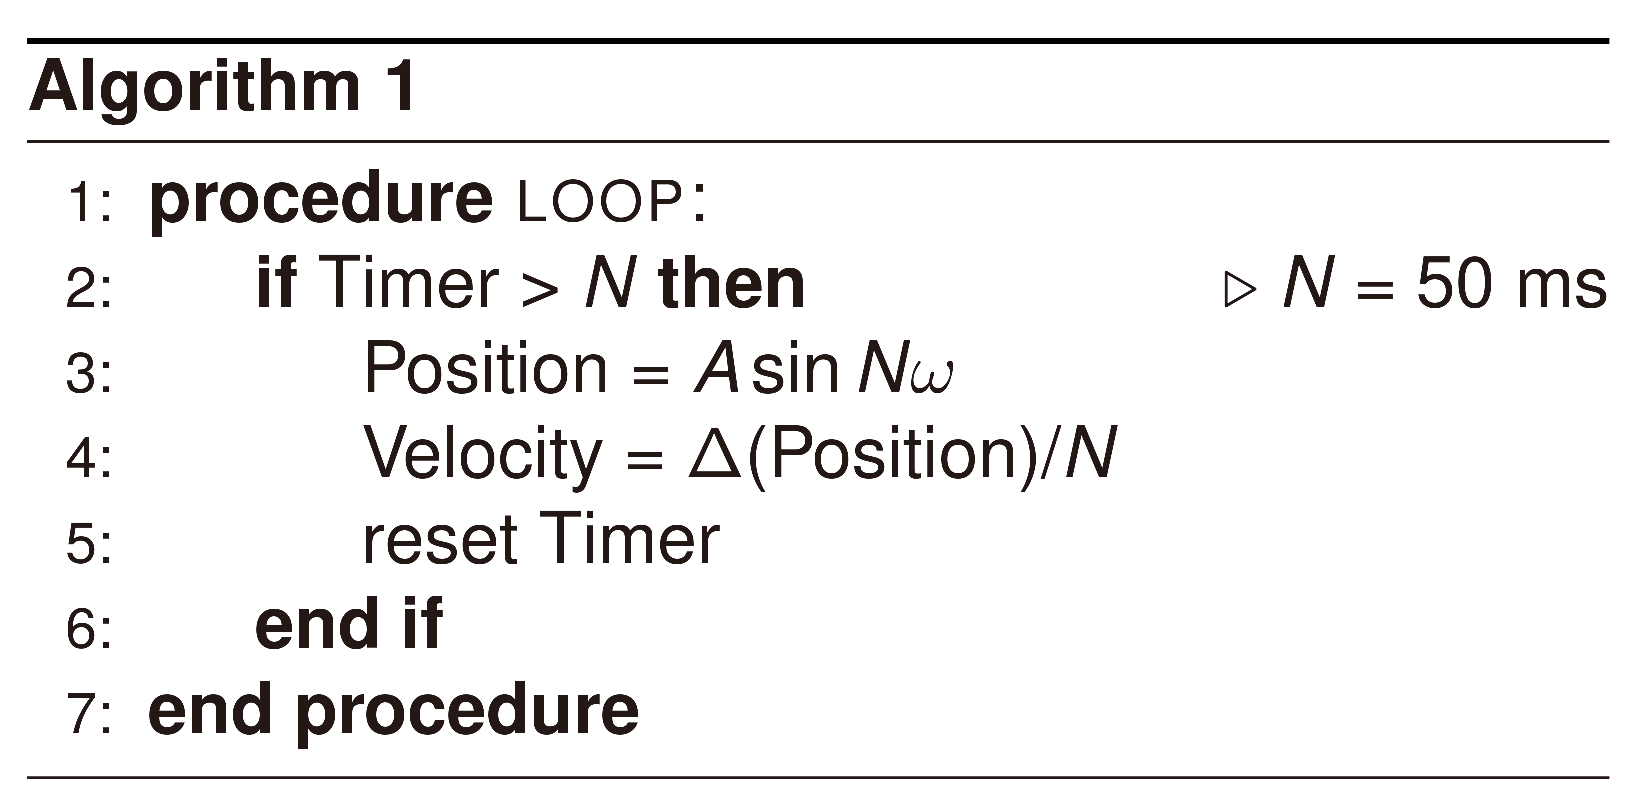
\includegraphics[width=0.38\textwidth]{images/algorithm.pdf} 
      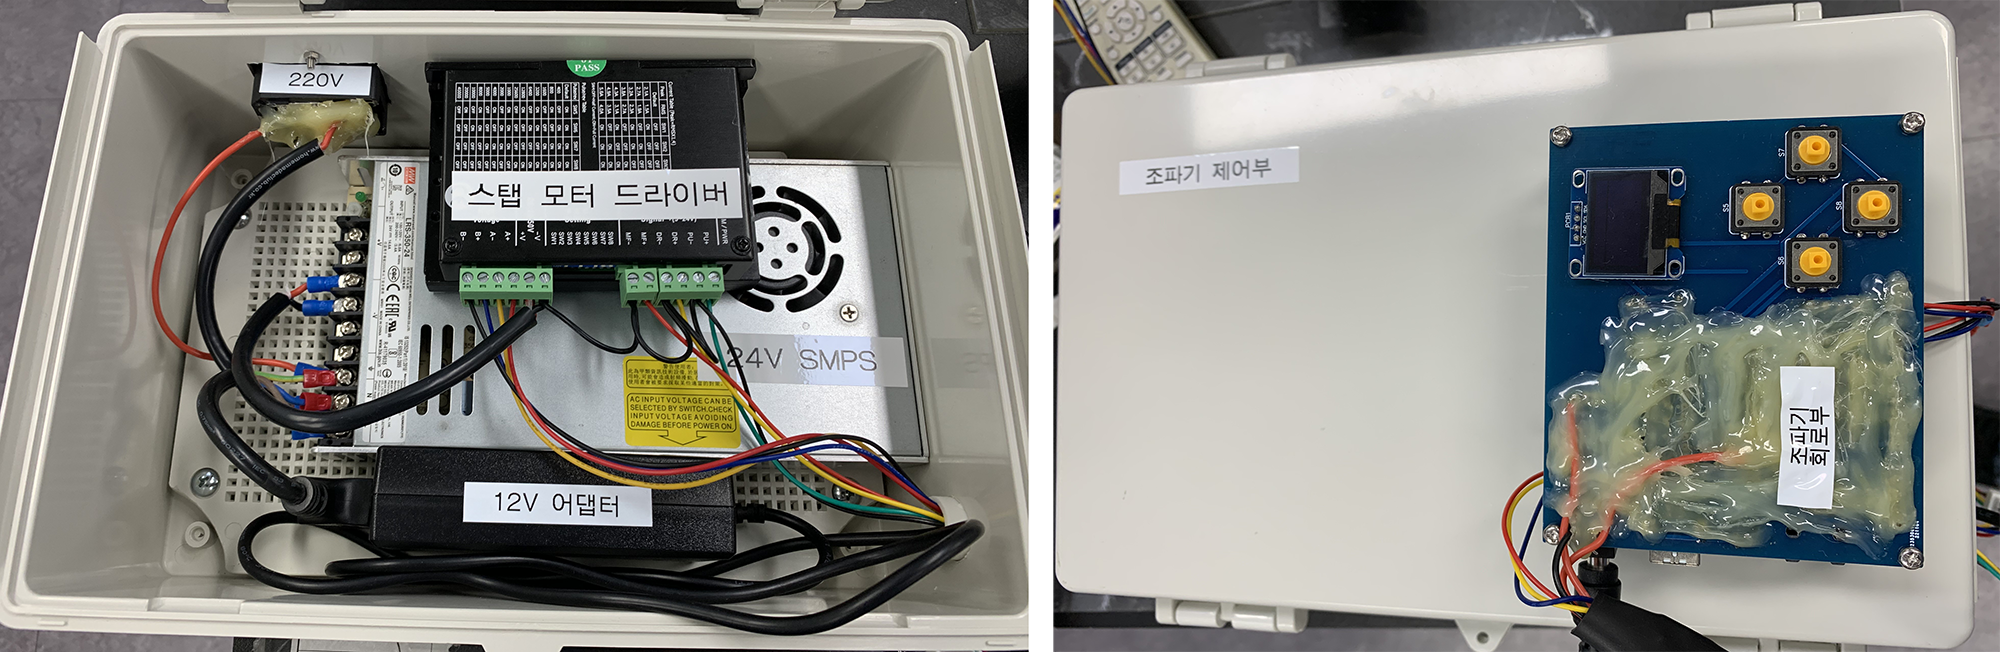
\includegraphics[width=0.62\textwidth]{images/made.png} 
        \captionof{figure}{code algorithm(좌), 모터 드라이버와 연결한 컨트롤 박스(우)}
     \label{algotithm}

\vspace{1.0em}
\small {4. OLED 디스플레이어 모습 \\}
    \scriptsize {
    
    버튼 스위치와 OLED 디스플레이어를 사용하여 메뉴를 구성하였다. 메뉴는 트리 형태의 구조를 이용해 구현하여 누구나 직관적으로 쉽게 조작할 수 있도록 코딩하였다. 이렇게 OLED 디스플레이어가 장착되어 있어 펌웨어가 업로드 되면 컴퓨터 없이도 손쉽게 파도를 생성할 수 있다는 것이 특장점 중의 하나이다. \\
    로고 화면에서 조파기가 끝점을 인식하는 것을 기다리면 메뉴 화면으로 들어간다. 메뉴에서는 규칙파, 불규칙파, 그리고 수동 조절을 선택할 수 있다. \\}
    
    %\begin{figure}[H]
            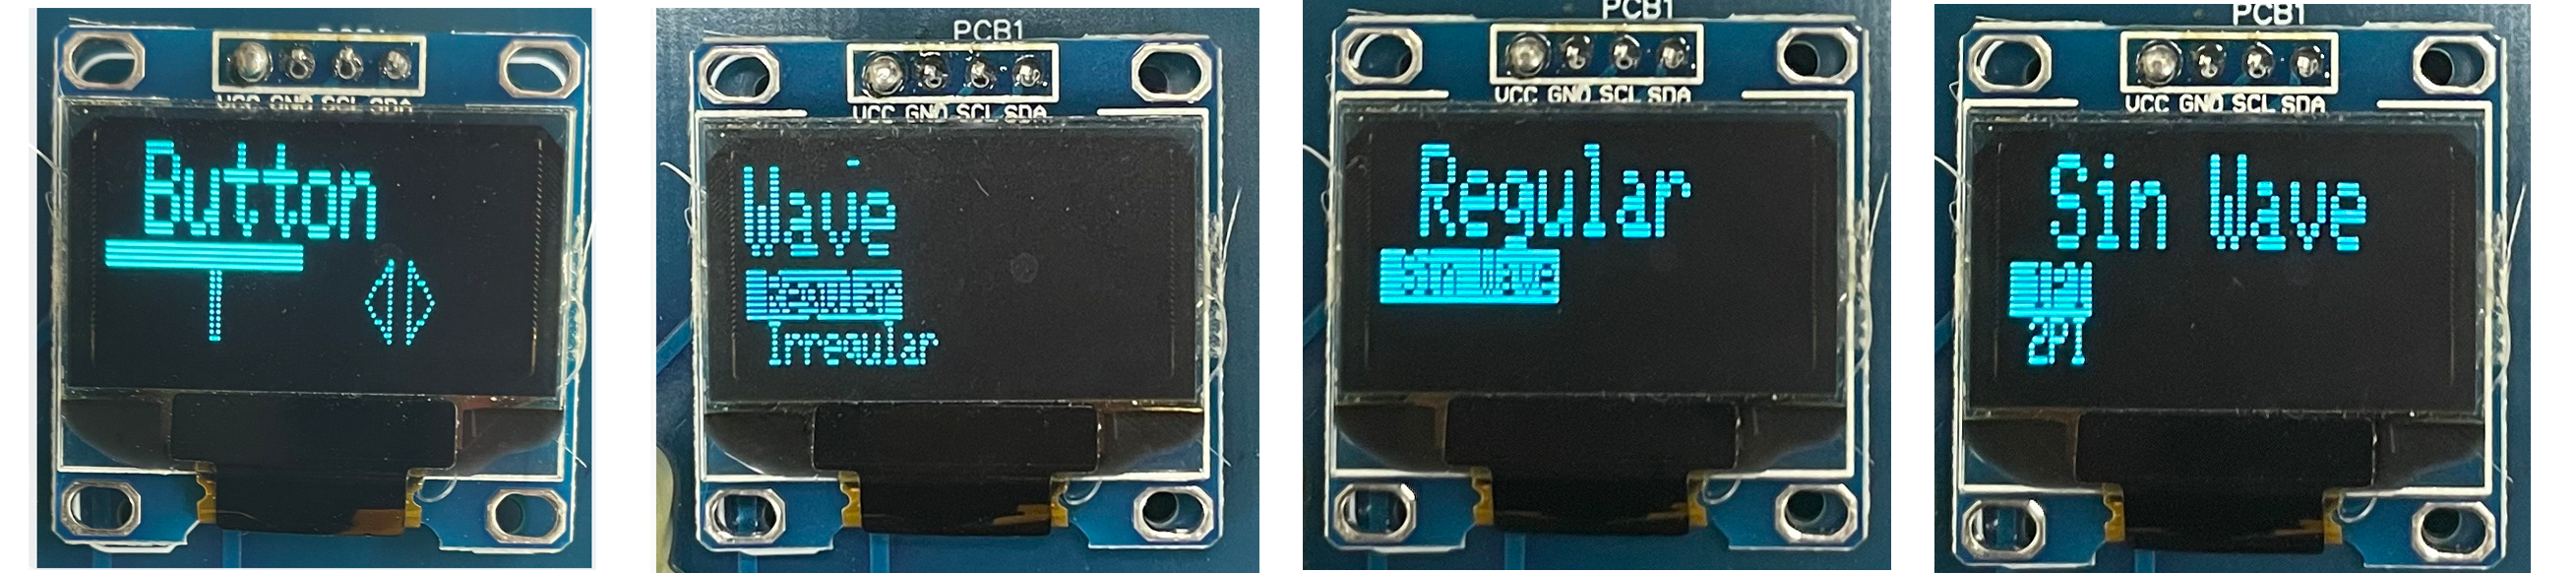
\includegraphics[width=\textwidth, height=1.5cm]{images/OLED.png} 
        \captionof{figure}{디스플레이 메뉴 동작 모습}
        \label{Oled}
\vspace{4.0em}
\end{posterbox}

\begin{posterbox}[name=wmaker,column=2, below=wtank] {작품 설명: C. 그 외} %, above=bottom-20em
\small {1. 소파 장치\\}
    \scriptsize {
    파는 수조 내부에서 전달되며 수조 말단에서 반사파가 생성된다. 중첩의 원리에 의하여 수면파는 진행파와 반사파에 의한 정상파의 선형 결합으로 표현되며 정상파가 주요 오차의 원인이 되므로 이를 방지하기 위해 소파장치가 필요하다.\\}

\small{2. 파고계\\}
    \scriptsize {
    파고를 측정하기 위하여 스티로품 부표를 이용하였다. 부표가 좌우로 움직이지 않도록 하기 위하여 스티로폼 가운데 두 개의 구멍을 뚫고 낚시줄을 이용하여 고정한 후 파가 진행할 때 부표의 상하 운동을 동영상으로 촬영하여 분석하였다.}
    
    %\begin{figure}[H]
        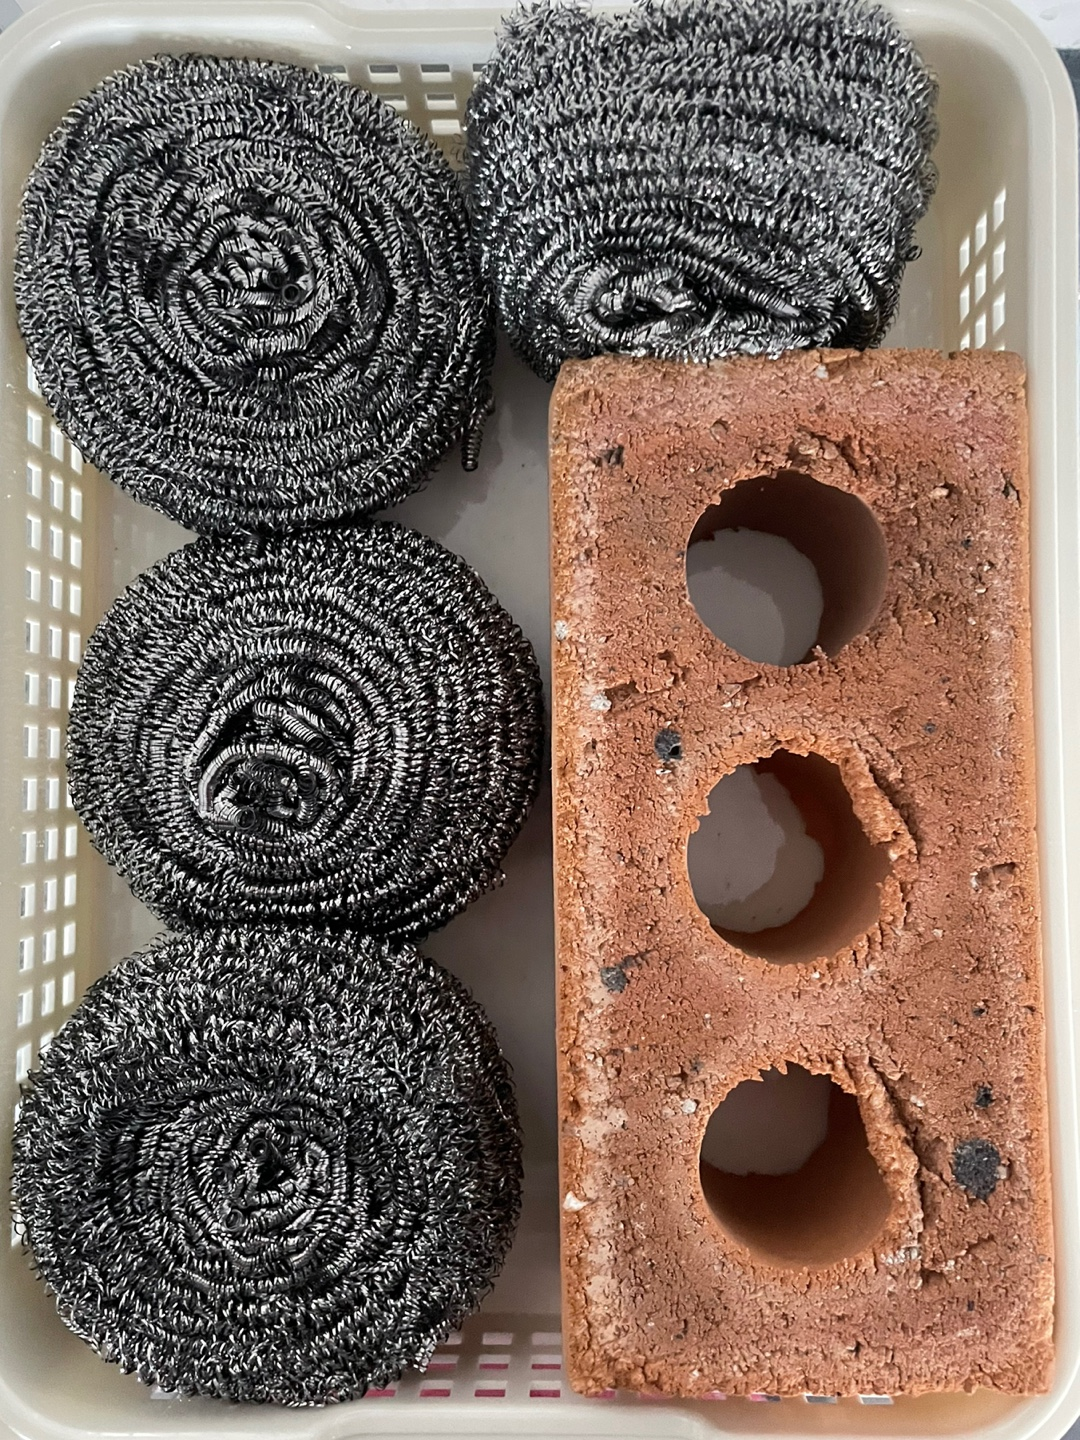
\includegraphics[width=0.3\textwidth, height=2.2cm]{images/sopagi2.jpg}
        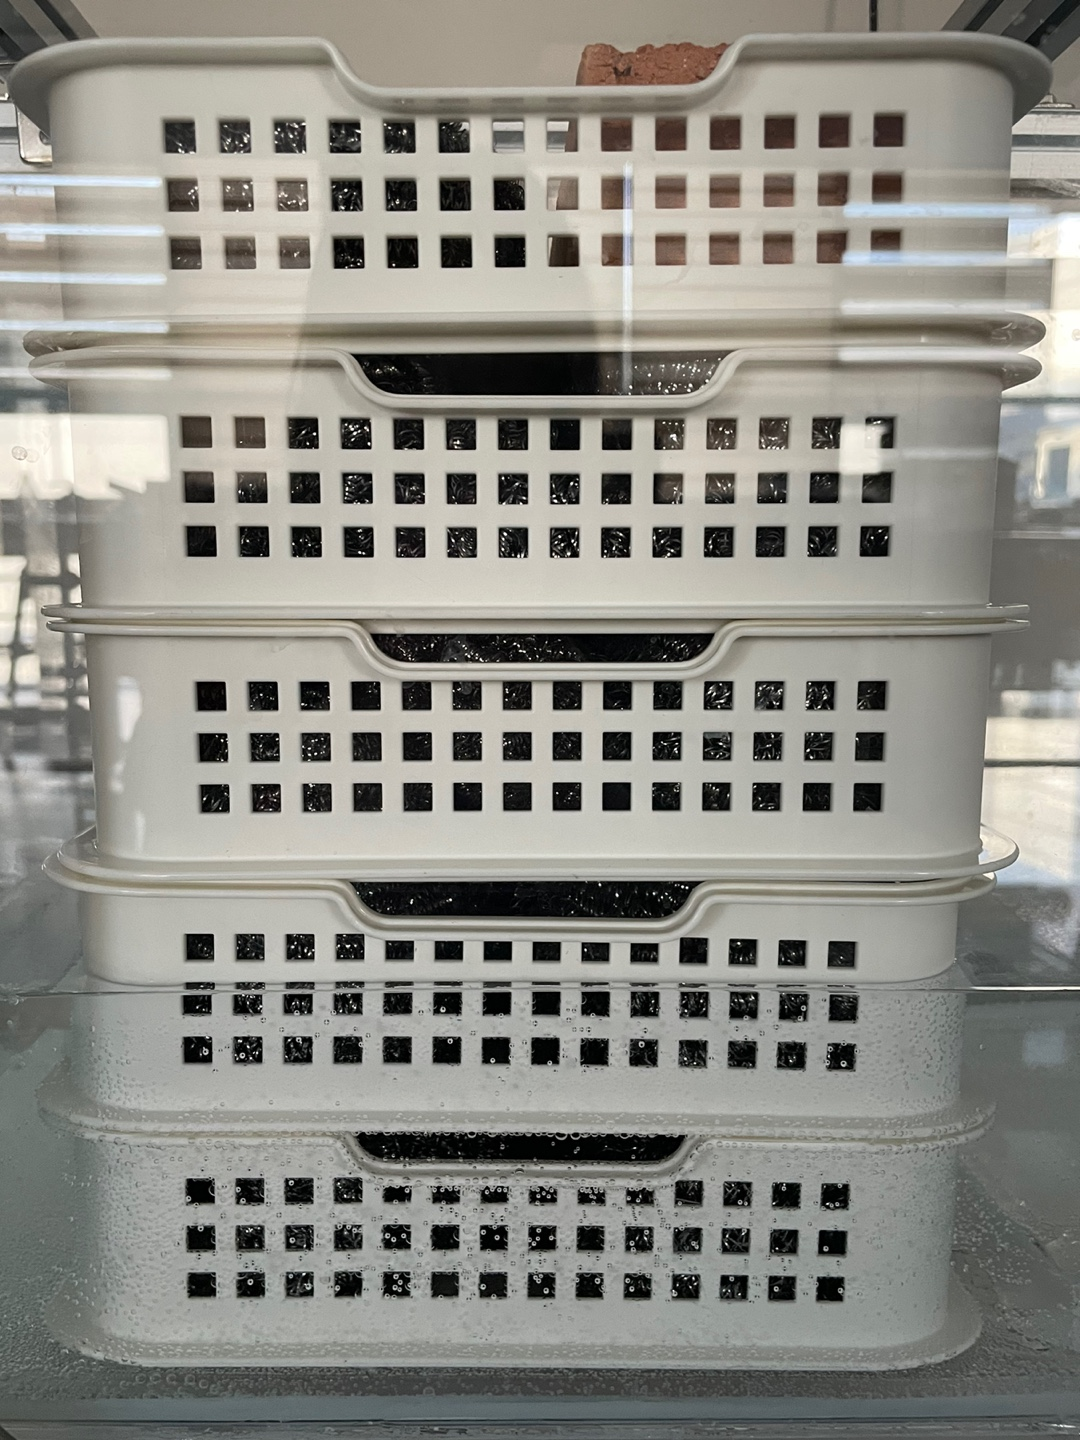
\includegraphics[width=0.3\textwidth, height=2.2cm]{images/sopagi1.jpg}
        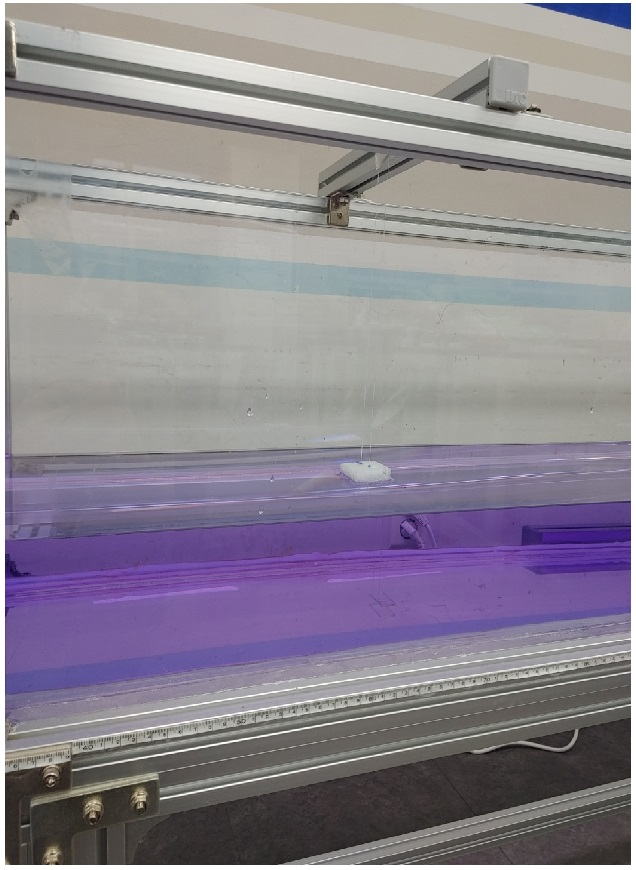
\includegraphics[width=0.375\textwidth, height=2.2cm]{images/Wave_Gauge.jpg}
        \captionof{figure}{(a) 플라스틱 바구니에 철수세미와 벽돌을 담은 모습, (b) 플라스틱 바구니를 수직으로 쌓아 올린 모습, (c) 파고를 측정하는 모습}
        %\captionof{figure}{완성된 조파수조의 모습}
        \label{wave absorb} 
        \begin{tikzpicture} [remember picture, overlay, anchor=north west, inner sep=0pt]
            \node [%draw=yellow, 
                    text=yellow,
                    ] at (0.1, 3.2) {\scriptsize{(a)}};
            \node [%draw=yellow, 
                    text=yellow,
                    ] at (2.5, 3.2) {\scriptsize{(b)}};
            \node [%draw=yellow, 
                    text=yellow,
                    ] at (5.0, 3.2) {\scriptsize{(c)}};
            \end{tikzpicture}	
    %\end{figure}
    
\small{3. 해안 경사\\}
    \scriptsize {
    해저에서 해안으로 이어지는 구조를 모형화 하여 해안 경사로를 설치할 수 있다. 긴 아크릴 판에 알루미늄 프로파일로 지지대를 만들어 높이와 기울기를 조절할 수 있도록 설계하였으며 그림 \ref{Coastal_Model(Ramp)} 속 경사로는 높이 $200\mathrm{~mm}$, 길이 $2,000\mathrm{~mm}$로 기울기가 1/10이다.}
    %\begin{figure}[H]
    \begin{center}
        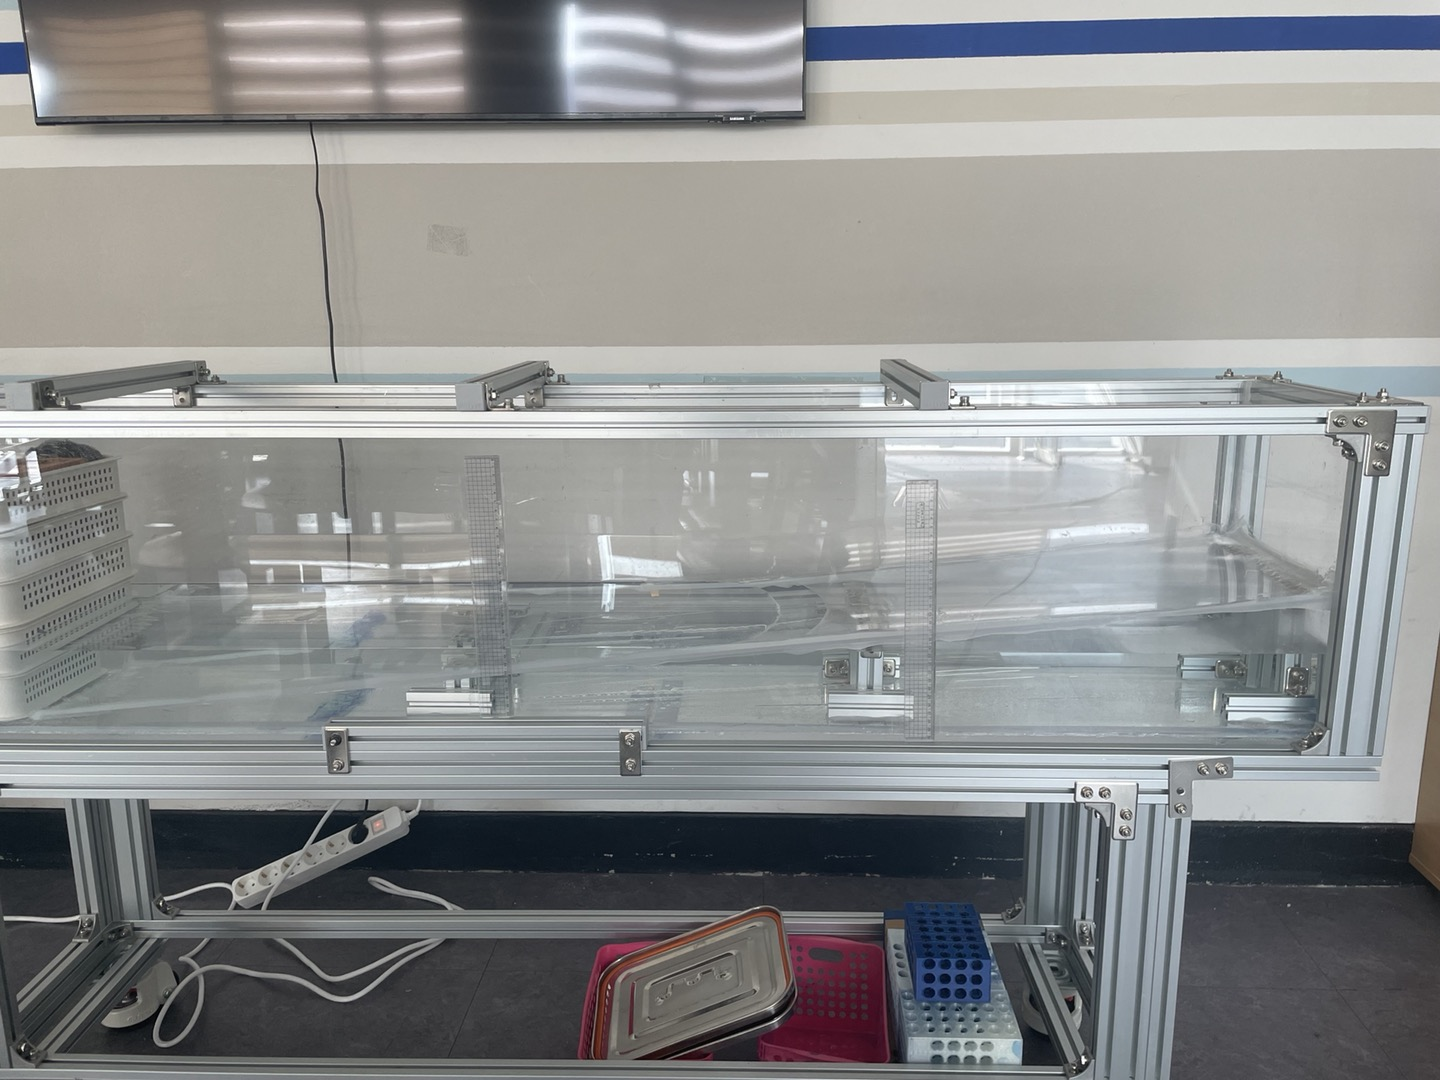
\includegraphics[trim=0 200 0 300, clip, 
            width=0.8\textwidth, 
            %height=1.2cm,
            ]
        {images/Coastal_Model(Ramp).jpg}
        \captionof{figure}{Coastal Model - Ramp}
        \label{Coastal_Model(Ramp)}
        \end{center}
    %\end{figure}

\end{posterbox}

\begin{posterbox}[name=result,column=3,]{결론  }

\small {1. 조파기 특성\\}

    \scriptsize{
    
        조파기 특성을 분석하기 위해 아래와 같이구동 코드의 매개 변수에 따른 판의 움직임과 생성되는 파를 관측하였다. //}

    %\begin{figure}[H]
    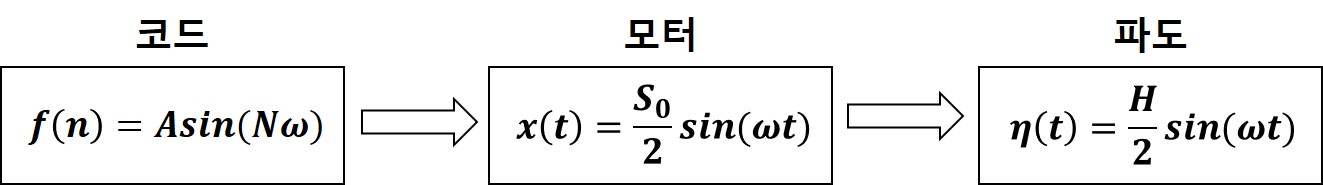
\includegraphics[width=.9\textwidth]{images/Flow_Chart(Analysis System_Kor).jpg}
    \captionof{figure}{조파기 검증 실험의 흐름도}
    \label{Flow_Chart}
    %\end{figure}
    
    \scriptsize{
    실험을 통해 구한 $H/S$는 Dean and Darlymple의 이론과는 달리 기울기가 1인 선형 관계를 만족하지 않았고 심해파 구간 ($\omega\sim4\pi$)에서도 잘 맞지 않았다. 이는 이론 전개의 여러 근사에 대한 조건을 충족하지 못하는 경우이다. 하지만 파형은 sin파에 근접하였고 Calibration을 통해 원하는 $H$에 대한 $S$를 지정할 수 있다. 또, $\omega$가 커질수록 모터에서 구현 가능한 진폭이 제한되어 있고 구현 가능한 스트로크의 범위를 알아야 한다. 단, 판과 파도, 코드에서 작성한 $\omega$는 모두 일치함을 확인하였고 조파기의 다른 매개변수를 조절하면 다양한 파를 생성할 수 있다. 추가적으로, 소파기의 성능 검증이 필요하며 무엇보다 연안 모형의 종류에 따라 여러 실험을 전개할 수 있다. \\}
  
    %\begin{figure}[H]
        \begin{filecontents}{HSthm-HSmsr.dat}
                HS_thm	HS_msr
                1.781440728	0.925436527
                1.785651376	1.085170025
                1.787735635	1.027713311
                1.782498659	1.045913291
                1.760671425	1.094309648
                1.787735635	1.15104453
                1.768471166	1.150212766
                1.77931432	1.26011236
                1.769571325	1.151819856
                1.776098332	1.252500343
                1.502818971	0.907053163
                1.512879552	1.042827713
                1.509535179	0.952282833
                1.51120852	0.957989748
                1.501134272	0.989520132
                1.526163172	1.182451424
                1.501302842	1.031007752
                1.502482211	0.900403351
                1.519540335	0.724198251
                1.501134272	0.877353529
                1.324569679	0.909190732
                1.324937643	0.929155313
                1.321072373	0.986915888
                1.323465588	1.024621212
                1.313331279	0.887096774
                1.315913161	0.964838394
                1.309086454	0.733436773
                1.326041332	0.895167286
                0.958556795	0.531089978
                0.958906454	0.580898876
                0.959081306	0.608042895
                0.958731617	0.530870712
                0.959081306	0.635545557
                0.956634768	0.607395324
                0.959431056	0.540311804
                0.95646013	0.524718468
                0.958556795	0.547893826
                0.954714602	0.645610278
                0.792888221	0.451327434
                0.792888221	0.377926685
                0.790392394	0.481381958
                0.793981875	0.44980695
                0.783557379	0.464839094
                0.791639619	0.434911243
                0.792419834	0.455155071
                0.79195164	0.393355983
                0.798366989	0.608601216
                0.800094292	0.48515625
                0.492276411	0.242943759
                0.528893957	0.280658651
                0.543862815	0.296883754
                0.553908234	0.308036891
                0.552905492	0.306913997
                0.542089448	0.294936947
                0.546948794	0.300287356
                0.551047756	0.304839279
                0.521368486	0.272679232
                0.499818992	0.25048407                  
            \end{filecontents}

            \begin{tikzpicture}[
                    %Environment Cfg.
                    font=\bfseries\sffamily,
                    ]
                    \begin{axis}[
                        width=0.8\textwidth,
                        height=3.8cm,
                        at={(0,0)},
                        ymin=0,
                        ymax=1.4,
                        xmin=0,
                        xmax=2,
                        grid=both,
                        minor tick num =5,
                        minor tick style={draw=none},
                        minor grid style={thin,color=black!10},
                        major grid style={thin,color=black!10},
                        %ylabel style={rotate=90},
                        ylabel={$H/S_{msr}$},
                        xlabel={$H/S_{thm}$},
                        tick align=outside,
                        axis x line*=middle,
                        axis y line*=none,
                        xtick={0,0.2,...,2},
                        ytick={0,0.2,...,2},
                        xlabel style={font=\sf\tiny},
                        ylabel style={font=\sf\tiny},
                        x tick label style={
                            /pgf/number format/assume math mode, font=\sf\tiny},
                        y tick label style={
                            /pgf/number format/assume math mode, font=\sf\tiny},
                        legend cell align = {left},
                        legend pos = north west,
                        legend style={nodes={scale=0.3, transform shape}},
                        ]
                        \addplot[scatter, 
                                only marks, 
                                mark=o,
                                mark size=0.5pt,
                                color=black,
                            ] 
                        table [x=HS_thm, y=HS_msr] {HSthm-HSmsr.dat};    
                        \addplot [thick, red] table [y={create col/linear regression={y=HS_msr}}] {HSthm-HSmsr.dat};
                        %\addlegendentry{$y(x)$}
                        \addlegendentry{
                            Linear regression: $ \omega_{msr} =
                            \pgfmathprintnumber{\pgfplotstableregressiona}
                            \cdot \omega_{thm}
                            \pgfmathprintnumber[print sign]{\pgfplotstableregressionb}$
                        };
                    \end{axis}
        \end{tikzpicture}
    \captionof{figure}{$H/S_{msr} - H/S_{thm}$ graph}
    \label{H/S graph}
    %\end{figure} 
    
\begin{filecontents}{acc.dat}
                t	y_30000	y_40000	y_50000
                0	0.19965	-0.0461	-0.70283
                0.033367	0.88578	0.79731	0.26519
                0.066734	1.41854	1.54643	1.3542
                0.1001	1.78019	2.09436	2.16649
                0.133467	2.10058	2.51832	2.74721
                0.166834	2.42496	2.9166	3.28632
                0.2002	2.65052	3.25279	3.73685
                0.233567	2.69128	3.32493	3.95223
                0.266934	2.69601	3.32011	4.0169
                0.3003	2.68381	3.31722	4.04341
                0.333667	2.53945	3.18505	3.92908
                0.367034	2.24984	2.85109	3.62093
                0.4004	1.94568	2.46075	3.19471
                0.433767	1.6103	2.00279	2.6843
                0.467134	1.14521	1.38601	1.98441
                0.5005	0.55864	0.64207	1.11098
                0.533867	-0.0586	-0.14149	0.16794
                0.567234	-0.68693	-0.94865	-0.8004
                0.6006	-1.16272	-1.669	-1.63958
                0.633967	-1.51151	-2.20274	-2.34206
                0.667334	-1.86959	-2.67197	-3.00563
                0.7007	-2.15706	-3.05802	-3.48397
                0.734067	-2.2686	-3.25109	-3.80335
                0.767434	-2.3295	-3.3759	-4.05893
                0.8008	-2.3925	-3.44363	-4.18022
                0.834167	-2.34221	-3.34345	-4.09689
                0.867534	-2.12824	-3.09611	-3.91013
                0.9009	-1.92868	-2.80851	-3.63691
                0.934267	-1.66742	-2.44389	-3.16259
                0.967634	-1.20691	-1.87777	-2.55154
                1.001	-0.71952	-1.22286	-1.84435
                1.034367	-0.20613	-0.50127	-1.04396
                1.067734	0.42368	0.31501	-0.09588
                1.1011	1.05093	1.12604	0.91296
                1.134467	1.51691	1.75337	1.7925
                1.167834	1.85038	2.20687	2.43867
                1.2012	2.15589	2.58406	3.00982
                1.234567	2.44035	2.96622	3.51607
                1.267934	2.55892	3.18147	3.8099
                1.3013	2.58132	3.1805	3.92574
                1.334667	2.58654	3.18082	3.99092
                1.368034	2.50032	3.12393	3.96888
                1.4014	2.27759	2.85251	3.70347
                1.434767	2.01037	2.44489	3.35212
                1.468134	1.70864	2.02859	2.9192
                1.5015	1.27966	1.48942	2.28589
                1.534867	0.72957	0.7975	1.52725
                1.568234	0.13968	-0.00332	0.65856
                1.6016	-0.46007	-0.82565	-0.34092
                1.634967	-1.00343	-1.61238	-1.27387
                1.668334	-1.39078	-2.12874	-1.98071
                1.7017	-1.73618	-2.63824	-2.67774
                1.735067	-2.05872	-3.06711	-3.25502
                1.768434	-2.2378	-3.33038	-3.59615
                1.8018	-2.28124	-3.46167	-3.88219
                1.835167	-2.35317	-3.55984	-4.08709
                1.868534	-2.34231	-3.52169	-4.05134
                1.9019	-2.18136	-3.3411	-3.88661
                1.935267	-1.96749	-3.06891	-3.67773
                1.968634	-1.71625	-2.72452	-3.26969
                2.002	-1.28602	-2.2191	-2.70558
                2.035367	-0.81728	-1.55728	-2.02746
                2.068734	-0.31872	-0.84745	-1.2709
                2.1021	0.26265	-0.07845	-0.30425
                2.135467	0.9496	0.788	0.72003
                2.168834	1.40154	1.52533	1.62134
                2.2022	1.75468	2.01573	2.30078
                2.235567	2.10147	2.46746	2.94581
                2.268934	2.3967	2.87079	3.47737
                2.3023	2.55238	3.15844	3.81726
                2.335667	2.62076	3.23622	4.00602
                2.369034	2.65914	3.27771	4.14932
                2.4024	2.58367	3.24675	4.15548
                2.435767	2.39857	3.05535	3.94408
                2.469134	2.17446	2.71809	3.62721
                2.5025	1.88444	2.34949	3.25509
                2.535867	1.49925	1.85688	2.65401
                2.569234	1.00332	1.21929	1.93541
                2.6026	0.44518	0.50017	1.14535
                2.635967	-0.19936	-0.3095	0.13966
                2.669334	-0.74776	-1.08519	-0.83255
                2.7027	-1.20231	-1.64584	-1.61405
                2.736067	-1.59977	-2.20759	-2.37864
                2.769434	-1.93983	-2.65238	-3.00176
                2.8028	-2.17932	-2.94288	-3.4264
                2.836167	-2.29458	-3.10488	-3.73815
                2.869534	-2.37942	-3.21108	-3.99138
                2.9029	-2.38288	-3.20642	-4.04015
                2.936267	-2.27697	-3.0282	-3.91074
                2.969634	-2.1216	-2.7839	-3.74705
                3.003	-1.91887	-2.45772	-3.3983
                3.036367	-1.55399	-1.99512	-2.917
                3.069734	-1.07152	-1.35359	-2.28586
                3.1031	-0.64736	-0.69868	-1.56226
                3.136467	-0.07503	0.07567	-0.67443
                3.169834	0.62139	0.96725	0.30019
                3.2032	1.15329	1.72133	1.32913
                3.236567	1.52816	2.28082	2.12527
                3.269934	1.89348	2.70848	2.72048
                3.3033	2.24371	3.18353	3.26412
                3.336667	2.43633	3.40231	3.70057
                3.370034	2.53906	3.47484	3.94051
                3.4034	2.60009	3.55977	4.05245
                3.436767	2.56799	3.57702	4.09095
                3.470134	2.42036	3.37121	3.96946
                3.5035	2.20923	3.07584	3.65483
                3.536867	1.93066	2.78252	3.2648
                3.570234	1.55913	2.26567	2.78462
                3.6036	1.10325	1.61979	2.07279
                3.636967	0.5802	0.97997	1.24147
                3.670334	-0.02334	0.17924	0.34297
                3.7037	-0.65857	-0.75173	-0.64667
                3.737067	-1.17285	-1.37792	-1.55053
                3.770434	-1.56799	-1.91885	-2.26503
                3.8038	-1.90164	-2.46202	-2.94488
                3.837167	-2.23698	-2.85342	-3.50423
                3.870534	-2.44391	-3.05384	-3.83199
                3.9039	-2.49569	-3.19402	-4.0644
                3.937267	-2.51034	-3.29516	-4.2654
                3.970634	-2.5445	-3.24324	-4.26093
                4.004	-2.42687	-3.03	-4.03252
                4.037367	-2.16947	-2.75013	-3.75746
                4.070734	-1.90945	-2.413	-3.36757
                4.1041	-1.51816	-1.933	-2.83599
                4.137467	-1.03935	-1.29424	-2.10184
                4.170834	-0.50818	-0.57231	-1.2709
                4.2042	0.06957	0.31284	-0.26666
                4.237567	0.73165	1.17361	0.75584
                4.270934	1.2455	1.87399	1.6875
                4.3043	1.58747	2.36544	2.40174
                4.337667	1.89112	2.73069	2.95997
                4.371034	2.16959	3.11726	3.35944
                4.4044	2.37204	3.38282	3.71815
                4.437767	2.4319	3.40654	3.89543
                4.471134	2.42094	3.3675	3.95554
                4.5045	2.3439	3.3302	3.92504
                4.537867	2.18696	3.1265	3.74224
                4.571234	1.92323	2.7545	3.39073
                4.6046	1.59431	2.28924	2.94849
                4.637967	1.21345	1.74871	2.39218
                4.671334	0.71115	1.12462	1.6625
                4.7047	0.12966	0.3269	0.79821
                4.738067	-0.47148	-0.51087	-0.16585
                4.771434	-1.05047	-1.27666	-1.12757
                4.8048	-1.49682	-1.80115	-1.92418
                4.838167	-1.82838	-2.27316	-2.58851
                4.871534	-2.17445	-2.71807	-3.17688
                4.9049	-2.43635	-3.04975	-3.62932
                4.938267	-2.48784	-3.21874	-3.86814
                4.971634	-2.51503	-3.29405	-4.06024
                5.005	-2.56856	-3.30492	-4.15906
                5.038367	-2.4869	-3.1784	-4.04501
                5.071734	-2.25169	-2.91066	-3.74639
                5.1051	-2.01171	-2.55853	-3.3832
                5.138467	-1.7465	-2.1082	-2.98582
                5.171834	-1.28108	-1.54368	-2.3775
                5.2052	-0.75679	-0.94807	-1.61234
                5.238567	-0.19342	-0.15545	-0.61791
                5.271934	0.41501	0.72147	0.35113
                5.3053	0.97708	1.50741	1.32609
                5.338667	1.38601	2.09393	2.13243
                5.372034	1.69529	2.46928	2.73626
                5.4054	1.9505	2.84432	3.30207
                5.438767	2.13855	3.19731	3.73049
                5.472134	2.23725	3.34286	4.02161
                5.5055	2.25088	3.2946	4.16939
                5.538867	2.18332	3.24129	4.16521
                5.572234	2.03225	3.17057	4.03556
                5.6056	1.80633	2.85472	3.7849
                5.638967	1.50978	2.36769	3.37659
                5.672334	1.12638	1.89813	2.83644
                5.7057	0.61015	1.3599	2.17771
                5.739067	0.09032	0.56945	1.35831
                5.772434	-0.51844	-0.26237	0.43367
                5.8058	-1.17384	-1.05176	-0.52577
                5.839167	-1.65163	-1.76004	-1.41355
                5.872534	-1.99282	-2.29776	-2.09461
                5.9059	-2.39362	-2.74567	-2.7724
                5.939267	-2.69534	-3.09648	-3.28198
                5.972634	-2.83697	-3.30478	-3.59474
                6.006	-2.97469	-3.43862	-3.80204
                6.039367	-3.04448	-3.47008	-3.97475
                6.072737	-2.96871	-3.40402	-3.96754
                6.106097	-2.80123	-3.19323	-3.7299
                6.139467	-2.578	-2.91812	-3.37793
                6.172837	-2.32669	-2.54115	-3.01313
                6.206197	-2.02032	-2.05056	-2.49922                    
            \end{filecontents}
        
            \begin{tikzpicture}[
                    %Environment Cfg.
                    font=\bfseries\sffamily,
                ]
                    \begin{axis}[
                        width=\textwidth,
                        height=3.8cm,
                        at={(0,0)},
                        ymin=-4.3,
                        ymax=4.3,
                        xmin=0,
                        xmax=7,
                        grid=both,
                        minor tick num =5,
                        minor tick style={draw=none},
                        minor grid style={thin,color=black!10},
                        major grid style={thin,color=black!10},
                        %ylabel style={rotate=90},
                        ylabel={$y~\left[\mathrm{cm} \right]$},
                        xlabel={$t~\left[\mathrm{s} \right]$},
                        tick align=outside,
                        axis x line*=middle,
                        axis y line*=none,
                        xtick={0, 2, 4, 6, 8},
                        ytick={-4, -2, 0, 2 ,4},
                        xlabel style={font=\sf\tiny},
                        ylabel style={font=\sf\tiny},
                        x tick label style={
                            /pgf/number format/assume math mode, font=\sf\tiny},
                        y tick label style={
                            /pgf/number format/assume math mode, font=\sf\tiny},
                        legend cell align = {left},
                        legend pos = north east,
                        legend style={at={(1,1)},anchor=north east},
                        legend style={nodes={scale=0.3, transform shape}},
                        ]
                        \addplot [%only marks, 
                            mark = +,
                            mark size=.5pt,
                            color=black,
                            ] 
                            table [x=t, y=y_30000] {acc.dat};
                        \addlegendentry{acc = 30000};
                        \addplot [%only marks, 
                            mark = *,
                            mark size=.5pt,
                            color=black,
                            ] 
                            table [x=t, y=y_40000] {acc.dat};
                        \addlegendentry{acc = 40000};
                        \addplot [%only marks, 
                            mark = o,
                            mark size=.5pt,
                            color=black,
                            ] 
                            table [x=t, y=y_50000] {acc.dat};
                        \addlegendentry{acc = 50000}; 
                    \end{axis}
        \end{tikzpicture}
    \captionof{figure}{가속도를 다르게 한 경우의 파고 데이터}
    \label{fig:diffa}
\\

\small {2. 파도 생성 모습\\}
    \scriptsize{
    
    조파기의 움직임으로 규칙파가 생성되는 모습을 촬영한 후 일부 프레임을 캡쳐하여 아래 그림에 나타내었다. 조파판의 움직임을 다르게 정밀 제어하면 여러 종류의 해파를 만들어 다양한 연안 환경 실험을 할 수 있을 것이다.\\}
    %\begin{figure}[H]
            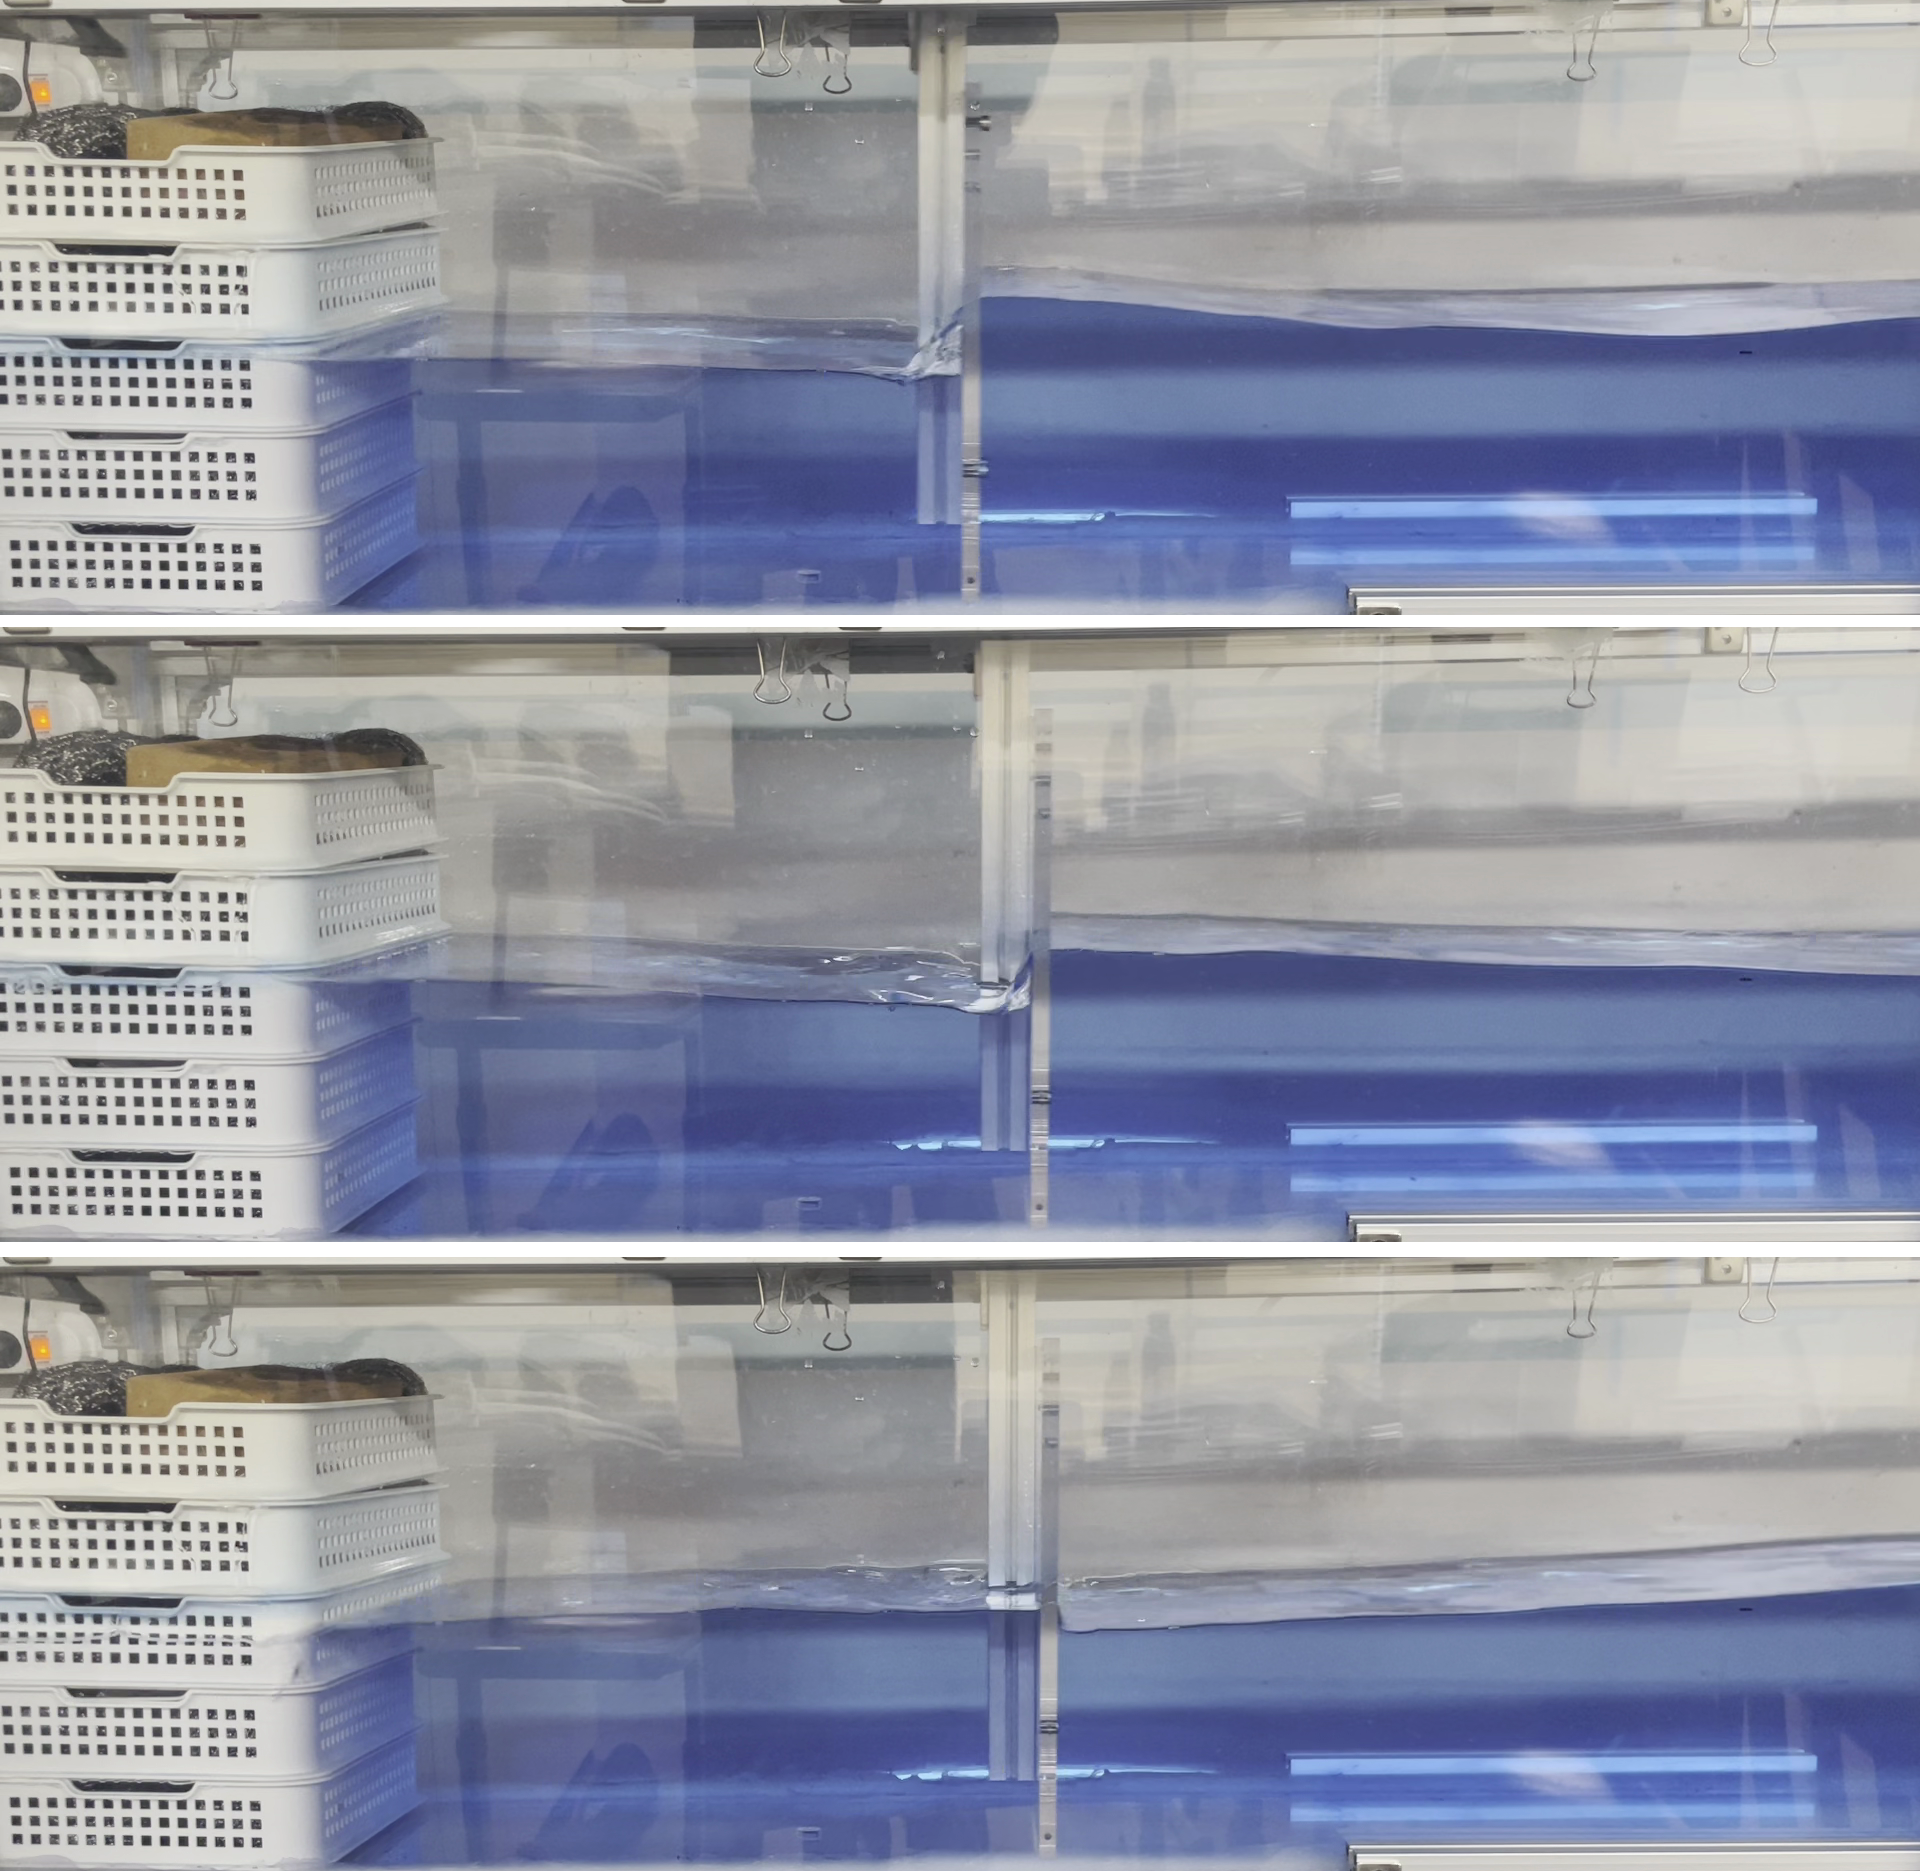
\includegraphics[trim=0 0 0 0, clip, width=0.49\textwidth, 
                height=3.8cm,
                ]
                {images/vlcsnap-2023-06-29-10h35m08s932-1.png} 
            % (왼쪽, 아래(), 오른쪽, 위(숫자가 클수록 위에서 많이 잘림) )
            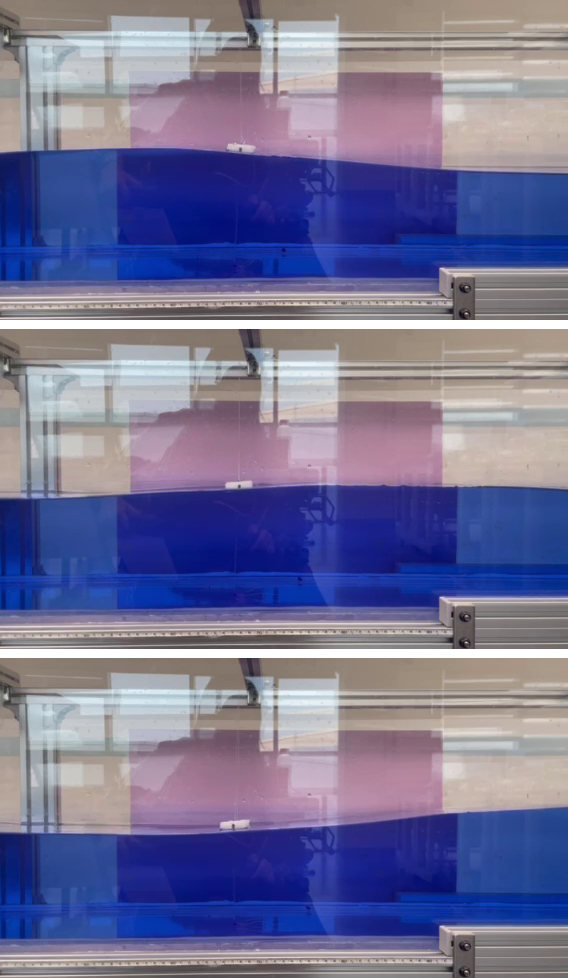
\includegraphics[trim=0 0 0 0, clip, width=0.49\textwidth, 
                height=3.8cm,
                ]
                {images/vlcsnap-2023-06-29-10h53m08s226-1.png} 
         \captionof{figure}{(a) 조파기로 파도를 만드는 동작 (b) 생성된 파도가 전파될때 파고를 측정하는 모습}
        \label{result}   
        \begin{tikzpicture} [remember picture, overlay, anchor=north west, inner sep=0pt]
            \node [%draw=yellow, 
                    text=yellow,
                    ] at (0.1, 4.7) {\scriptsize{(a)}};
            \node [%draw=yellow, 
                    text=yellow,
                    ] at (4, 4.7) {\scriptsize{(b)}};
         \end{tikzpicture}	 
    %\end{figure}    
\end{posterbox}

\begin{posterbox}[name=refs,column=3,below=result]{참고문헌}
%\scriptsize
\tiny
\bibliographystyle{IEEEtran}
\bibliography{bibfile.bib}
\end{posterbox}

\end{poster}
\end{document}
